\newcommand{\BL}{D}
\newcommand{\CH}[1]{c(#1)}
\newcommand{\LB}[1]{l_{#1}}
\newcommand{\LBh}{n_l}
\newcommand{\NV}{N}
\newcommand{\RBh}{n_r}
\newcommand{\RN}{\psi}
\newcommand{\RNALL}{\Psi}
\newcommand{\SD}{\omega}
\newcommand{\SDALL}{\Omega}
\newcommand{\TBL}{L}
\newcommand{\TO}{T^\SD}
\newcommand{\TR}{T^\RN}
\newcommand{\TRO}{\TR_{\SD}}
\newcommand{\bl}{\delta}
\newcommand{\child}[2]{#1_{#2}}
\newcommand{\defeq}{=}
\newcommand{\la}{\lambda_a}
\newcommand{\lb}{\lambda_b}
\newcommand{\li}{\lambda_i}
\newcommand{\leaf}{\otimes}
\newcommand{\tav}{\tau'}
\newcommand{\tO}{t^\SD}

\newtheorem{conjecture}{Conjecture}
\newtheorem{corollary}{Corollary}
\newtheorem{lemma}{Lemma}
\newtheorem{theorem}{Theorem}

%% START DUAL-BIRTH CHAPTER
\chapter{\dualbirthtitle}
\label{chap:dualbirth}
\clearpage

Models of tree evolution have mostly focused on capturing the cladogenesis processes behind speciation. Processes that derive the evolution of genomic elements, such as repeats, are not necessarily captured by these existing models. In this paper, we design a model of tree evolution that we call the dual-birth model, and we show how it can be useful in studying the evolution of short \textit{Alu} repeats found in the human genome in abundance. The dual-birth model extends the traditional birth-only model to have two rates of propagation, one for active nodes that propagate often, and another for inactive nodes, that with a lower rate, activate and start propagating. Adjusting the ratio of the rates controls the expected tree balance. We present several theoretical results under the dual-birth model, introduce parameter estimation techniques, and study the properties of the model in simulations. We then use the dual-birth model to estimate the number of active \textit{Alu} elements and their rates of propagation and activation in the human genome based on a large phylogenetic tree that we build from close to one million \textit{Alu} sequences.

\section{Introduction}
Phylogenetic trees can be used to study the evolution of not just species, but of any sequence that evolves. For example, multi-copy gene families~\cite{Page1997,Finn2014}, cancer genomes~\cite{Nowell1976,El-Kebir2016}, antibodies~\cite{Litman1993,Robinson2015,Safonova2015}, segmental duplicates~\cite{Bailey2006,Jiang2007}, and long or short interspersed nuclear elements~\cite{Dewannieux2003} are all biological sequences that evolve, and many of these evolve \textit{within} the genome of a single species. The process of diversification for many evolving entities can be characterized by propagation: an original copy of a sequence creates a new copy, and the two copies evolve independently by accumulating mutations. Phylogenetics provides a natural framework for studying such processes, but several challenges present themselves.

Given sufficiently long sequences and assuming our models of sequence evolution are reasonably accurate, we can recover the phylogenetic trees from sequence data with high accuracy~ \cite{Felsenstein2003,Roch2010}. However, unlike species-tree reconstruction, in which the entire genome can be used, reconstructing phylogenies of gene families, repeats, or antibodies is limited by the length of the evolving entity. As a result, high levels of uncertainty are to be expected in trees reconstructed from these types of sequences. These inherent limitations make accurate modeling of underlying processes crucial, perhaps even more so than species-tree reconstruction.

Models of tree evolution describe probability distributions over the space of tree shapes ~\cite{Yule1925,Brown1994,Aldous2001} and are useful in several ways. They can be used as the prior distribution in a Bayesian inference~\cite{Drummond2007,Mooers2012,Sayyari2016}. They can also generate null distributions describing certain neutral evolutionary process, which may then be rejected by trees inferred from the data~\cite{Guyer1991,Kirkpatrick1993,Agapow2002}. Moreover, the diversification parameters are inherently of interest to the biologist~\cite{Morlon2014}. Two well-known models of tree evolution are Yule (birth-only), in which each branch splits by a Poisson process with a constant rate, and birth-death, in which, in addition to birth, branches can go extinct with a constant rate. Each of these models have limitations and have inspired the development of several alternative models~\cite{Aldous1996,Steel2001,Ford2005,Blum2006,Jones2011,Maddison2007}.

A main feature of a tree evolution model is the expected tree shape, especially the tree balance (Fig.~\ref{fig:dualbirth-model}). The Yule model generates relatively balanced trees~\cite{McKenzie2000}, more so than typically seen in phylogenetic trees~\cite{Blum2006}. Some systems, such as certain viruses, are especially known to have very unbalanced trees~\cite{Volz2013}. Most models of evolution are exchangeable, meaning that, after a split, the two branches are indistinguishable. When evolution works in a series of propagation events (i.e., where an element copies itself), there is a natural way in which one of the child branches corresponds to the parent branch~\cite{Lambert2013}. The new copy may have properties that are different from the original branch, and as a result, non-exchangeable models may be more appropriate. For example, the new child may be initially incapable of propagation until it \textit{activates}. In such situations, the tree will tend to be unbalanced. In the limit, if every new child is impotent, one would expect a \textit{caterpillar}-like tree (Fig.~\ref{fig:dualbirth-model}).

In this paper, we study a non-exchangeable extension of the Yule model, which we name the dual-birth model. Each branch will split with one of two available rates. Branches that correspond to elements that have in the past propagated are considered \textit{active} and have a high rate of future propagation, whereas  branches that have never propagated are considered \textit{inactive}. With some rate, the Unlike some previous models (e.g. BiSSE~\cite{Maddison2007}), after every birth event, one of the two children inherits the parent's rate while the other child has the opposite rate (i.e., the model is asymmetric in the terminology of Lambert and Stadler (2013)~\cite{Lambert2013}). For this dual-birth  model, we describe methods for sampling the tree distribution, derive probability distributions on the tree space, compute the expectation of various tree statistics, and introduce methods of estimating the model parameters from data. In extensive simulations, we study the behavior of the model and our estimators. We then use the model to study the evolution of \textit{Alu} elements in the human genome.

\textit{Alu} elements are a family of \glspl{SINE}, each approximately 300 \gls{bp} long, that abound in the genomes of supraprimates and that retrotranspose via \gls{RNA} polymerase III-encoded \glspl{RNA}~\cite{Dewannieux2003}. There are approximately one million \textit{Alu} elements in the human genome, meaning they comprise roughly 10\% of the human genome. Although \textit{Alu} elements have no known biological function of their own~\cite{Schmid2003}, studying and understanding their retrotransposition in the genome can provide key insight into their contributions to genetic disease~\cite{Deininger1999} as well as useful information in the study of supraprimate evolution~\cite{Stoneking1997,Singer2003,Watkins2003}.

A topic of interest regarding \textit{Alu} elements is the number and identity of repeats that are capable of propagating through retrotransposition~\cite{Cordaux2004,Liu2009,Konkel2015}. Various hypotheses range from the single source model to the transposon model, where all elements are assumed to be equal in their ability to propagate~\cite{Cordaux2004}. We approach this question using phylogenetics and the dual-birth model. We build a tree for close to one million \textit{Alu} elements. Using the properties of the dual-birth model, we estimate the number of \textit{Alu} elements that have been active and estimate the rates of \textit{Alu} propagation and activation.

\section{Materials and Methods}
\subsection{Dual-Birth Model}
The dual-birth model is similar to the Yule process, but unlike Yule, it is not \textit{exchangeable}, meaning that left and right branches are not generated using identical processes. The dual-birth model is parameterized by two birth parameters: $\la$ and $\lb$. The generative process starts with a single root node, which immediately splits into two child branches \textit{left}, denoted by $a$,  and \textit{right}, denoted by $b$. Further birth events occur on each child branch according to a Poisson process with the constant rate $\la$ on branch $a$ and the constant rate $\lb$ on branch $b$. Thus, \textit{left} and \textit{right} are governed by different rates. Each new node becomes the root of an identical process. The process can be terminated at any point in time. This generates an unlabeled \textit{ordered}, also known as oriented~\cite{Lambert2013}, tree: each branch is labeled as either \textit{left} or \textit{right} (Fig.~\ref{fig:dualbirth-model}a). We define $r=\la/\lb$ and $\lambda=\la+\lb$, which together identify $\la$ and $\lb$. When $r=1$, the dual-birth process is reduced to the Yule process
with a rate of $\lambda/2$.

\subsubsection{Active/Inactive Elements}
Consider a tree in which each branch corresponds to some entity, and the right child of any branch corresponds to the same entity as the parent. Thus, each split is a propagation of the parent entity. Moreover, entities are either \textit{active} or \textit{inactive}. A branch is active if it has produced an offspring before and is otherwise considered inactive. The right child of any branch is always active while the left one is  inactive. Active entities  propagate with rate $\lb$ (for ``birth''), and inactive entities activate and simultaneously propagate with rate $\la$ (for ``activation''). Note that activation and the first propagation occur together (an alternative model could be that nodes activate mid-branch and wait for a birth event). Once an entity activates, it remains active (thus, there is no deactivation).

The dual-birth model can easily capture this scenario. If $r=1$ (i.e., the Yule model), active and inactive nodes have the same rates of birth, and thus, their difference is inconsequential. When $r<1$, new entities activate (i.e., propagate for the first time) with a rate $\la$ that is lower than the rate $\lb$ with which nodes that are already active propagate (Fig.~\ref{fig:dualbirth-model}b). Allowing $\la > \lb$ would result in $r > 1$, which yields a model that is non-identifiable with the model that has rate $1/r$. Setting $r>1$ would correspond to a scenario where the rate of propagation \textit{reduces} after the first activation, and we don't know of any scenario that justifies such reductions. Thus, our model defines $\la\leq\lb$ to remain identifiable.

One application of the dual-birth model is to study \textit{Alu} elements, though the model may prove useful for other systems, such as retroviruses or gene families. Each \textit{Alu} element appears at a specific position in the genome, and via retrotransposition, it can create a new copy of itself elsewhere in the genome, leading to a split in the repeat evolutionary tree. Each branch of the tree can thus be labeled by a position in the genome, which is the site at which the corresponding element resides. One child branch inherits the same position as the parent (and is thus active), and the other branch is the new copy, which is assumed to be initially inactive. The inactive state captures the observation that most \textit{Alu} elements don't propagate~\cite{Batzer2002}. The model allows for the chance that some inactive elements become active and start propagating, perhaps due to mutations or due to changes in their genomic context.

\subsubsection{Tree Balance}
The Yule model generates balanced trees, more so than trees typically found in phylogenetic databases~\cite{Guyer1991,Blum2006,Jones2011}. Similar to several other models of tree evolution~\cite{Aldous1996,Blum2006,Maddison2007}, the dual-birth model provides a natural way to control tree balance (we provide an extensive comparison to other models in the Discussion section). Consider an extreme case in which only one element is ever active. The resulting tree is a caterpillar, which will include only one cherry (an internal node is called a cherry if both of its children are leaves, i.e., terminal nodes). This outcome can be naturally achieved in dual-birth by setting $\la=0$ (i.e., $r=0$). When we expect to have many more inactive nodes than active nodes, we would still expect to see an unbalanced tree with few cherries. This outcome, too, can be achieved by a natural choice of $\la\ll\lb$, which results in $r\ll 1$. As $r$ increases, the tree becomes gradually more balanced (Fig.~\ref{fig:dualbirth-model}b). With $r=1$, the tree is as balanced as expected under the Yule model.

\begin{figure} % FIGURE 1 IN ORIGINAL PAPER
\centering
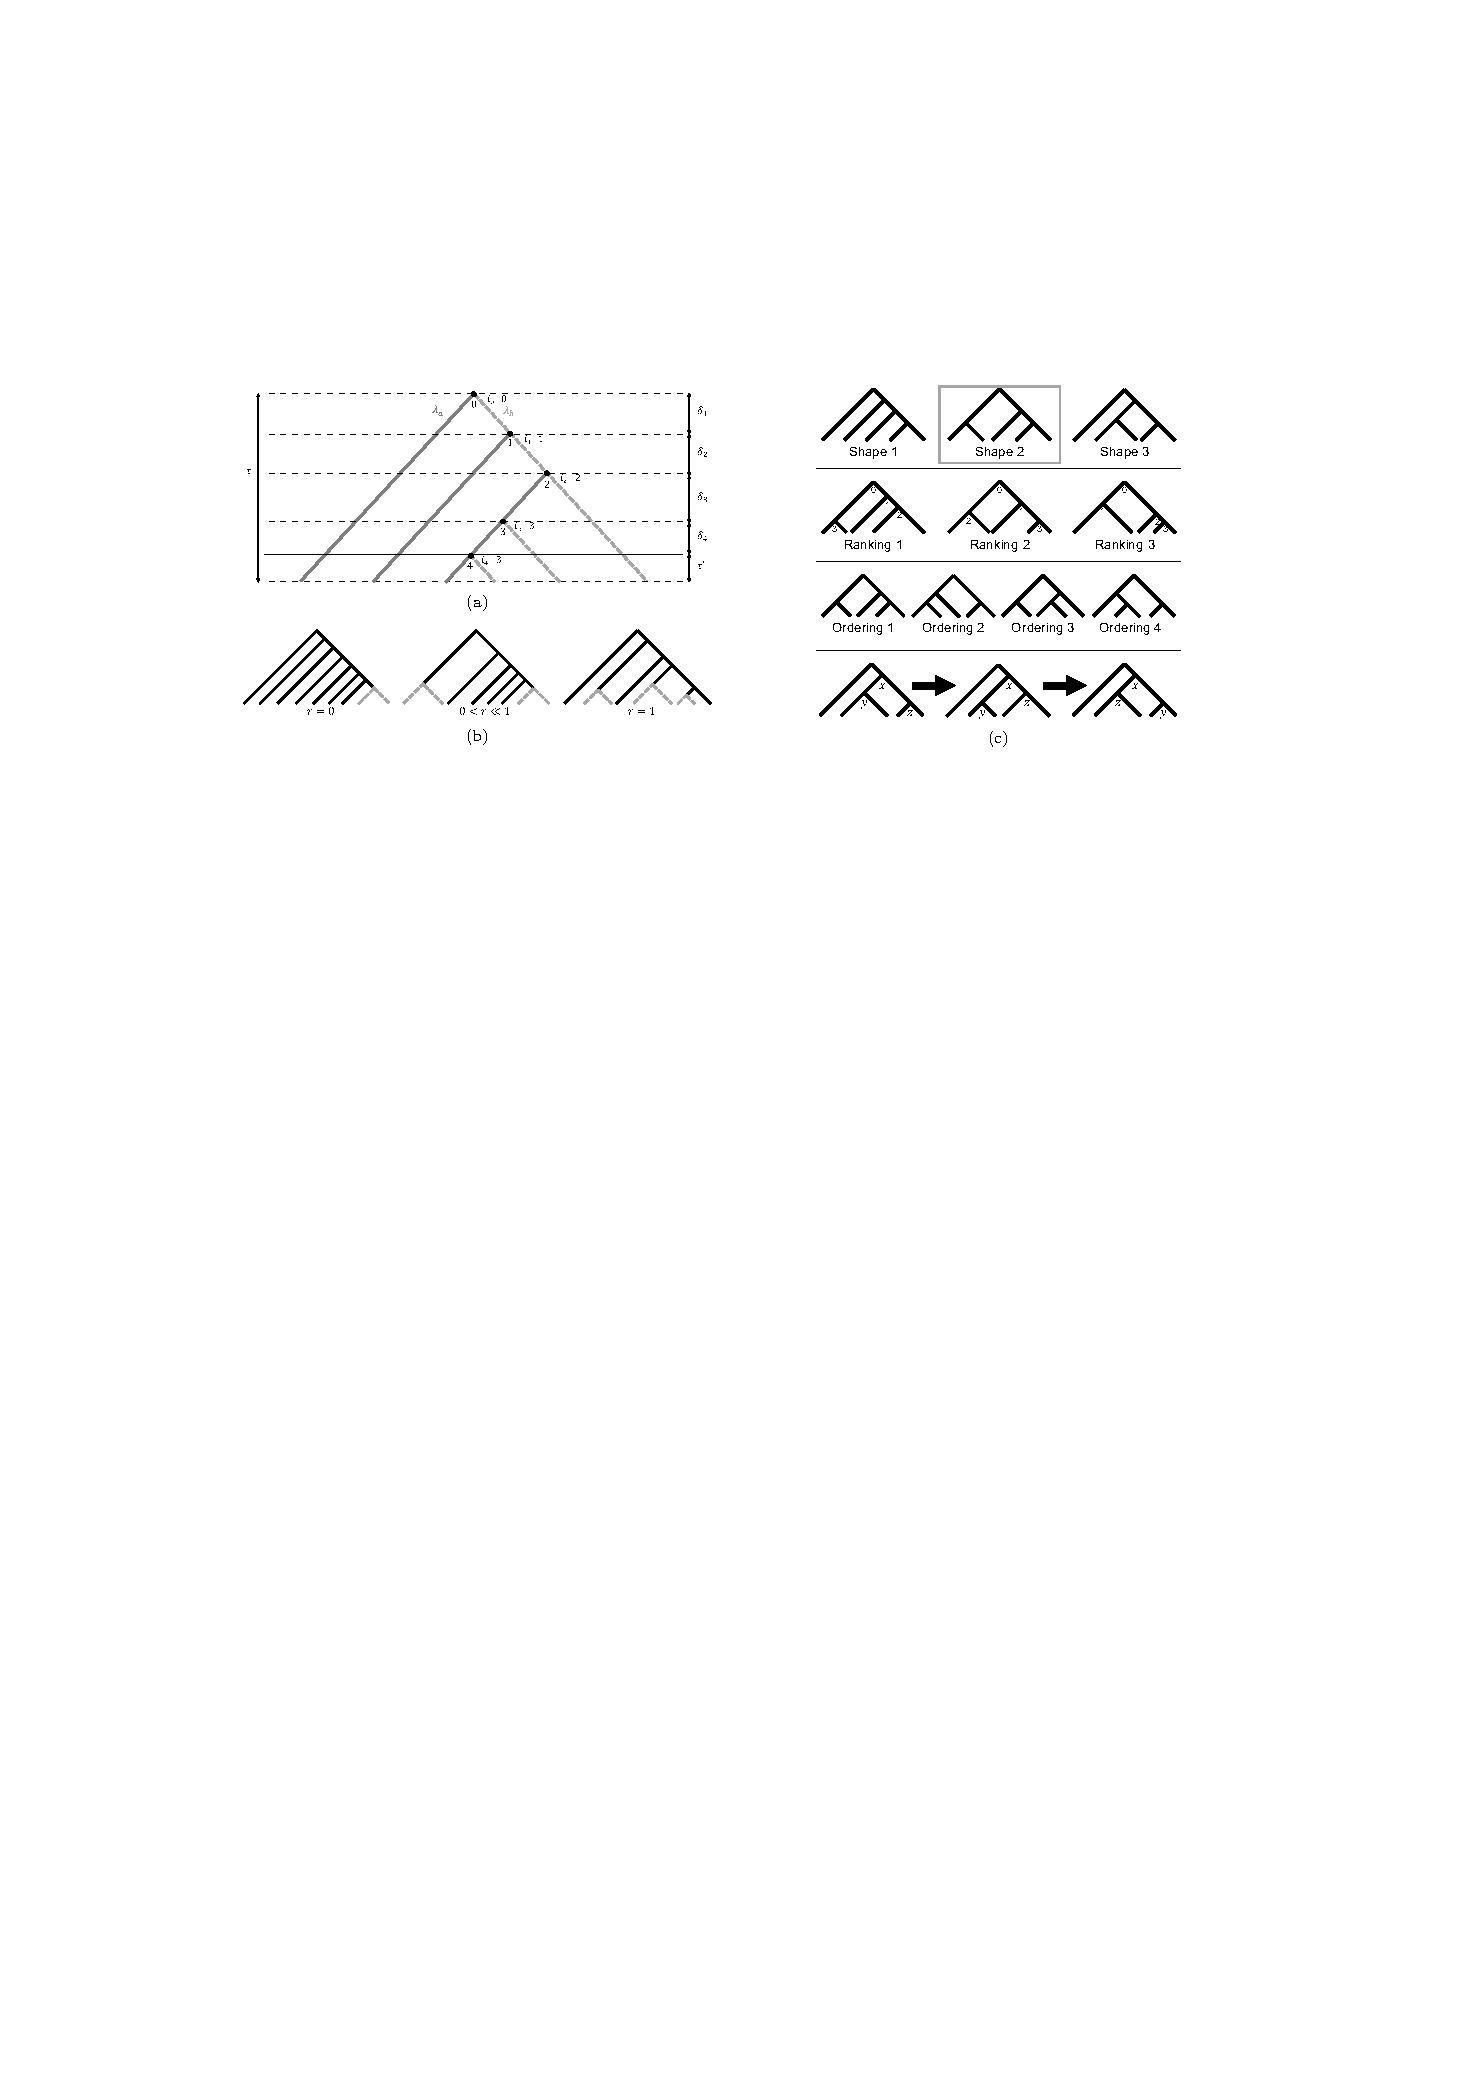
\includegraphics[width=\textwidth]{figs/dualbirth-model}
\caption[Dual-birth model]
{Dual-birth model. (a) A caterpillar tree with one cherry (node 4). The tree is generated by the dual-birth model; right branches (dashed light gray) are sampled from the Poisson process with rate $\lb$, and left branches (solid dark gray) are sampled with rate $\la$. Internal nodes are ranked by distance to the root (ranks shown below nodes), and the tree is divided into time intervals between consecutive nodes. (b) With $r=\la/\lb=0$, only caterpillar trees can be generated; as r increases toward $1$, the tree becomes more balanced and thus has more cherries (dashed light gray). (c) All three possible tree shapes with five leaves are shown on top; the second row shows $\RNALL$, all possible rankings of tree shape 2; the third row shows $\SDALL$, all orderings of tree shape 2. The last row demonstrates that, starting from a ranked ordered tree, one change of ranking followed by a change of ordering results in a tree identical to the original tree.}
\label{fig:dualbirth-model}
\end{figure}

\subsection{Theoretical Properties of the Dual-Birth Model}\label{sec:dualbirth-meth}
\subsubsection*{Notations and definitions}
A connected \gls{DAG} with no undirected cycles defines a tree. We only consider binary trees in which all nodes either have outdegree zero (leaves) or two (internal nodes). Two trees are considered to have the same \textit{shape} if there exists a one-to-one mapping between their nodes such that the head and tail of every edge in one tree map to the head and tail of exactly one edge in the other tree. In this paper, we care about the space of distinct tree shapes. In the tree-shape space, leaves are not distinguished (i.e., a tree shape is unlabeled). For simplicity of presentation, we represent a tree shape on $n$ leaves using $T=(V,E)$, where $V$ is the set of $n-1$ \textit{internal} nodes and $E$ is the set of internal edges $(u,v)$ from parent node $u$ to child node $v$. Note that terminal edges (connecting internal nodes to leaves) and leaves are not part of $E$ and $V$, and as such, are implicit in the $T$ formulation (each internal node has to have outdegree two). We use $\child{u}{1}$ and $\child{u}{2}$ to denote the children of $u$, and we use $\leaf$ to denote a generic unlabeled leaf. Note that $T$  defines a \gls{POSET} on $V$.

Recall a node $v\in V$ is called a cherry if both of its children are leaves. A tree shape is called \textit{caterpillar} if it has only one cherry (Fig.~\ref{fig:dualbirth-model}a); in contrast, a fully-balanced tree has exactly $n/2$ cherries. The number of cherries of a tree is denoted as $\CH{T}$.

Let $\NV\defeq\{0,1,\ldots, n-2\}$. A bijective function $\RN:V\mapsto\NV$ is a ranking of a tree $T=(E,V)$  if for each edge $(u,v)\in E$, we have $\RN(u)<\RN(v)$. A \textit{ranked tree shape} is defined as $\TR\defeq (T,\RN)$. Each ranking is a topological sorting of the tree (i.e., is a linear extension of the \gls{POSET} defined by the tree shape). We use $\RNALL(T)$ to denote the set of all possible rankings of the tree shape $T$ (Fig.~\ref{fig:dualbirth-model}c).

An \textit{ordered tree shape} is a tree shape in which left and right child nodes are distinguished (i.e., the tree is oriented). More precisely, $\SD:V\mapsto\{0,1\}$  is a valid order for a tree shape $T$ iff $\SD(\child{u}{1})+\SD(\child{u}{2})=1$ for every $(u,\child{u}{1}),(u,\child{u}{2})\in E$ and $\SD(r)=1$ for the root node $r$. We call $v$ a left child/node when $\SD(v)=0$ and otherwise call it a right child/node. A branch leading to a left (right) child is called a left (right) branch. An ordered tree shape is denoted by $\TO\defeq(T,\SD)$. Note that, in this definition, leaves are not directly assigned a left/right side. Leaves below a cherry are indistinguishable; leaves that are sister to internal nodes are considered to have the opposite side of their sibling. For example, in Figure~\ref{fig:dualbirth-model}a, the leaf directly below the root is considered a left node because its sister, the node ranked 1, is a right node. Also, $\SDALL(\TR)$ denotes the set of all possible orderings that are valid for $\TR$ (Fig.~\ref{fig:dualbirth-model}c).

A ranked ordered tree shape is defined by $\TRO\defeq(T,\RN,\SD)$. For ease of notation, we define $\SD_i\defeq\SD\left(\RN^{-1}(i)\right)$ (the order of the node ranked $i$). For $0<i<n$ and the ranked ordered tree $\TRO$, we define $\LB{i}(\TRO)\defeq1+\sum_{k=1}^{i-1}\SD_k$ and it is easy to show that $\LB{i}(\TRO)$ gives the number of left branches $(u,v)$ with $\SD(u) < i$ and $\SD(v) \geq i$. In other words, $\LB{i}(\TRO)$ gives the number of left terminal branches if the tree $\TRO$ is terminated at the time when node $i$ is created. Where clear by the context, we simply write $\LB{i}$ (Fig.~\ref{fig:dualbirth-model}a). We define $\LBh\defeq\LB{n-1}$ and $\RBh\defeq n-\LBh$; these definitions can be intuitively considered to show the number of left and right terminal branches, respectively, if we assign an order to all terminal branches (e.g. $\RBh=\LBh=3$ in Fig.~\ref{fig:dualbirth-model}a).

We refer to a tree shape with ultrametric branch lengths as a weighted shape. A weighted shape is defined by $t\defeq(T,\bl,\tau)$, where $\bl:E\mapsto\mathbb{R}$ gives the length of internal branches and $\tau$ gives the distance from the root to all leaves; note that $\tau$ has to be larger than the largest distance to the root from any internal node. Node ages define a unique ranking on any weighted shape. A weighted shape $t$ can also be assigned an order, $\SD$, and will be denoted by $\tO$. For $e=(u,v)\in E$, we refer to  $\bl(e)$ by $\bl_i$ where $i={\RN(v)}$ (e.g. $\bl_1\ldots\bl_4$ in Fig.~\ref{fig:dualbirth-model}a).

\subsubsection{Probability Distributions}
We now derive probability distributions on tree shapes conditioning on fixed $n$. Here we give the main results and provide the proofs in Section~\ref{sec:dualbirth-proofs}.

\begin{theorem}\label{thm:TRO}
Let $X$ be a random variable (r.v.) over ordered ranked tree shapes and distributed according to the dual-birth model with parameter $r=\la/\lb$. Then, 
\begin{equation}\label{eq:orts}
\Pr(X=\TRO;n) = \frac{r^{\RBh-1}}{\prod_{i=1}^{n-2} \big((r-1)\LB{i}+i+1\big)}
\end{equation}
\end{theorem}

Computing Equation~\ref{eq:orts} simply requires knowing the number of right leaves ($\RBh$) and the number of its left branches if the tree is terminated at each node $i$ ($\LB{i}$); all of these can be computed in time $O(n)$ for an ordered tree. Figure~\ref{fig:dualbirth-tree-prob-dists} shows the perfect match between Equation~\ref{eq:orts} and observed frequencies in simulations for all ranked ordered tree shapes with $n=6$ and shows that, with $r\ll1$, the caterpillar tree shape has a high probability.

The left/right order of nodes cannot be estimated from sequence data, and thus, it would be more useful to compute the probability distribution over unordered ranked tree shapes. Since all orderings of a \textit{ranked} tree are distinct, the probability of a ranked tree simply needs to marginalize over all possible orderings. Thus,
\begin{corollary}
For $Y$, an r.v.\ over ranked tree shapes with $n$ leaves and distributed according to the dual-birth model,
\begin{equation}\label{eq:rts}
\Pr(Y=\TR;n) = \sum_{\SD\in\SDALL(\TR)} \Pr(\TRO)
\end{equation}
where $\SDALL$ gives the set of all orderings of $\TR$.
\end{corollary}

This computing requires an exponential number of computations to iterate all orderings (the recursive formula for that iteration is given in Equation~\ref{sup:eq:sdall}. Whether efficient algorithms for computing this probability exist is unclear to us. See Figure~\ref{fig:dualbirth-tree-prob-dists} for an example distribution and matching simulations.

Next, we turn to computing the probability distribution over unranked shapes. This can be done by enumerating all possible rankings of the unranked tree and summing up their probabilities. The set of all rankings, $\RNALL(T)$, is simply the set of all the linear extensions of the \gls{POSET} defined by the tree shape. However, a final complication needs to be addressed. Recall that leaves are unlabeled. For a non-cherry symmetric node $u$ (i.e., sub-tree shapes below $\child{u}{1}$ and $\child{u}{2}$ are identical), take any ordering of any ranking of nodes below $u$. Now swap $\SD(\child{u}{1})$ and  $\SD(\child{u}{2})$ and also swap the rankings of nodes below $\SD(\child{u}{1})$ with the rankings of the identical nodes under $\SD(\child{u}{2})$ (Fig.~\ref{fig:dualbirth-model}c); this would produce an identical tree shape. However, our process will count this identical tree shape twice. To account for this, we need to divide the total probability by two for every non-cherry symmetric node. Thus,
\begin{corollary}
For $Z$, an r.v.\ over tree shapes with $n$ leaves and distributed according to the dual-birth model,
\begin{equation}\label{eq:rt}
\Pr(Z=T;n) = \frac{1}{2^{\sigma(T)}}\sum_{\RN\in\RNALL(T)} \Pr(\TR)
\end{equation}
where $\RNALL$ gives all rankings of $T$ and $\sigma(T)$ is the number of non-cherry symmetric nodes in $T$.
\end{corollary}

\subsubsection{Weighted Trees}
Given an ordered weighted tree shape $\TRO$, we can easily compute the probability density function (p.d.f) for the length of each of its internal branches. Recall $\bl_i$ is the time between internal nodes ranked $i-1$ and $i$ (i.e., an interval), which is simply the length of a specific branch. Given the tree shape, $\bl_i$  follows an exponential distribution with rate $\li=\la\LB{i}+\lb(i+1-\LB{i})$. This is because the branch length is simply the  minimum of all exponential r.v.s active in the corresponding interval, which itself, is an exponential r.v. with the total rate. Furthermore, since each interval is independent of the other intervals given $\TRO$, the joint probability density of $\TRO$ and a set of internal branch lengths can be computed by multiplying the probability of $\TRO$ (Eq.~\ref{eq:orts}) by the probability density of every branch length given $\TRO$. Finally, to compute the joint probability density of a given tree and all its branch lengths, we need to also multiple the probability of no births in the final interval of length $\bl_{n-1}=\tau-\sum_1^{n-2}\bl_{i}$; this is the probability of no events for an exponential with rate $\LB{n-1}$ in time $\bl_{n-1}$; i.e., $e^{-\LB{n-1}\bl_{n-1}}$.

\subsubsection{Expected Number of Cherries and Active Leaves}\label{sec:cherries}
We now ask the following question: how many cherries and how many active nodes are expected in a dual-birth tree generated with rate ratio $r$?

A parsimony analysis is constructive here. Activation events can be considered evolutionary changes. Given an unordered tree, the most parsimonious ordering is one that implies the minimum number of activation events. The number of activations is simply the number of left branches that have children. By making every internal node that is sister to a leaf a right node and arbitrarily ordering the rest, one can show that the most parsimonious ordering has exactly one activation for each cherry in the tree, counting the root as an activation (Lemma~\ref{lem:cherryparsimony}). The parsimony analysis would only be relevant for $r\ll1$, when one would expect very few activations. As $r$ increases, the tree becomes more balanced, and we would expect more cherries. We now formalize this intuition.

\begin{theorem}\label{thm:cherr}
For a tree shape $Z$ generated by the dual-birth model with $r=\la/\lb$, let $C=\CH{Z}/n$ be an r.v. capturing the fraction of cherries; then, 
\begin{align}\label{eq:cherries}
\lim_{n\to\infty}\mathbb{E}(C) = \frac{\sqrt{r}}{1+r+\sqrt{r}}
\end{align}
\end{theorem}

\begin{corollary}\label{cor:rbh}
For an r.v.\ $N_r$ capturing the fraction of right (i.e., active) leaves in tree shape $T$,
\begin{align}\label{eq:nr}
\lim_{n\to\infty}\mathbb{E}(N_r) = \frac{\sqrt{r}}{1+\sqrt{r}}
\end{align}
\end{corollary}

\begin{figure} % FIGURE 2 IN ORIGINAL PAPER
\centering
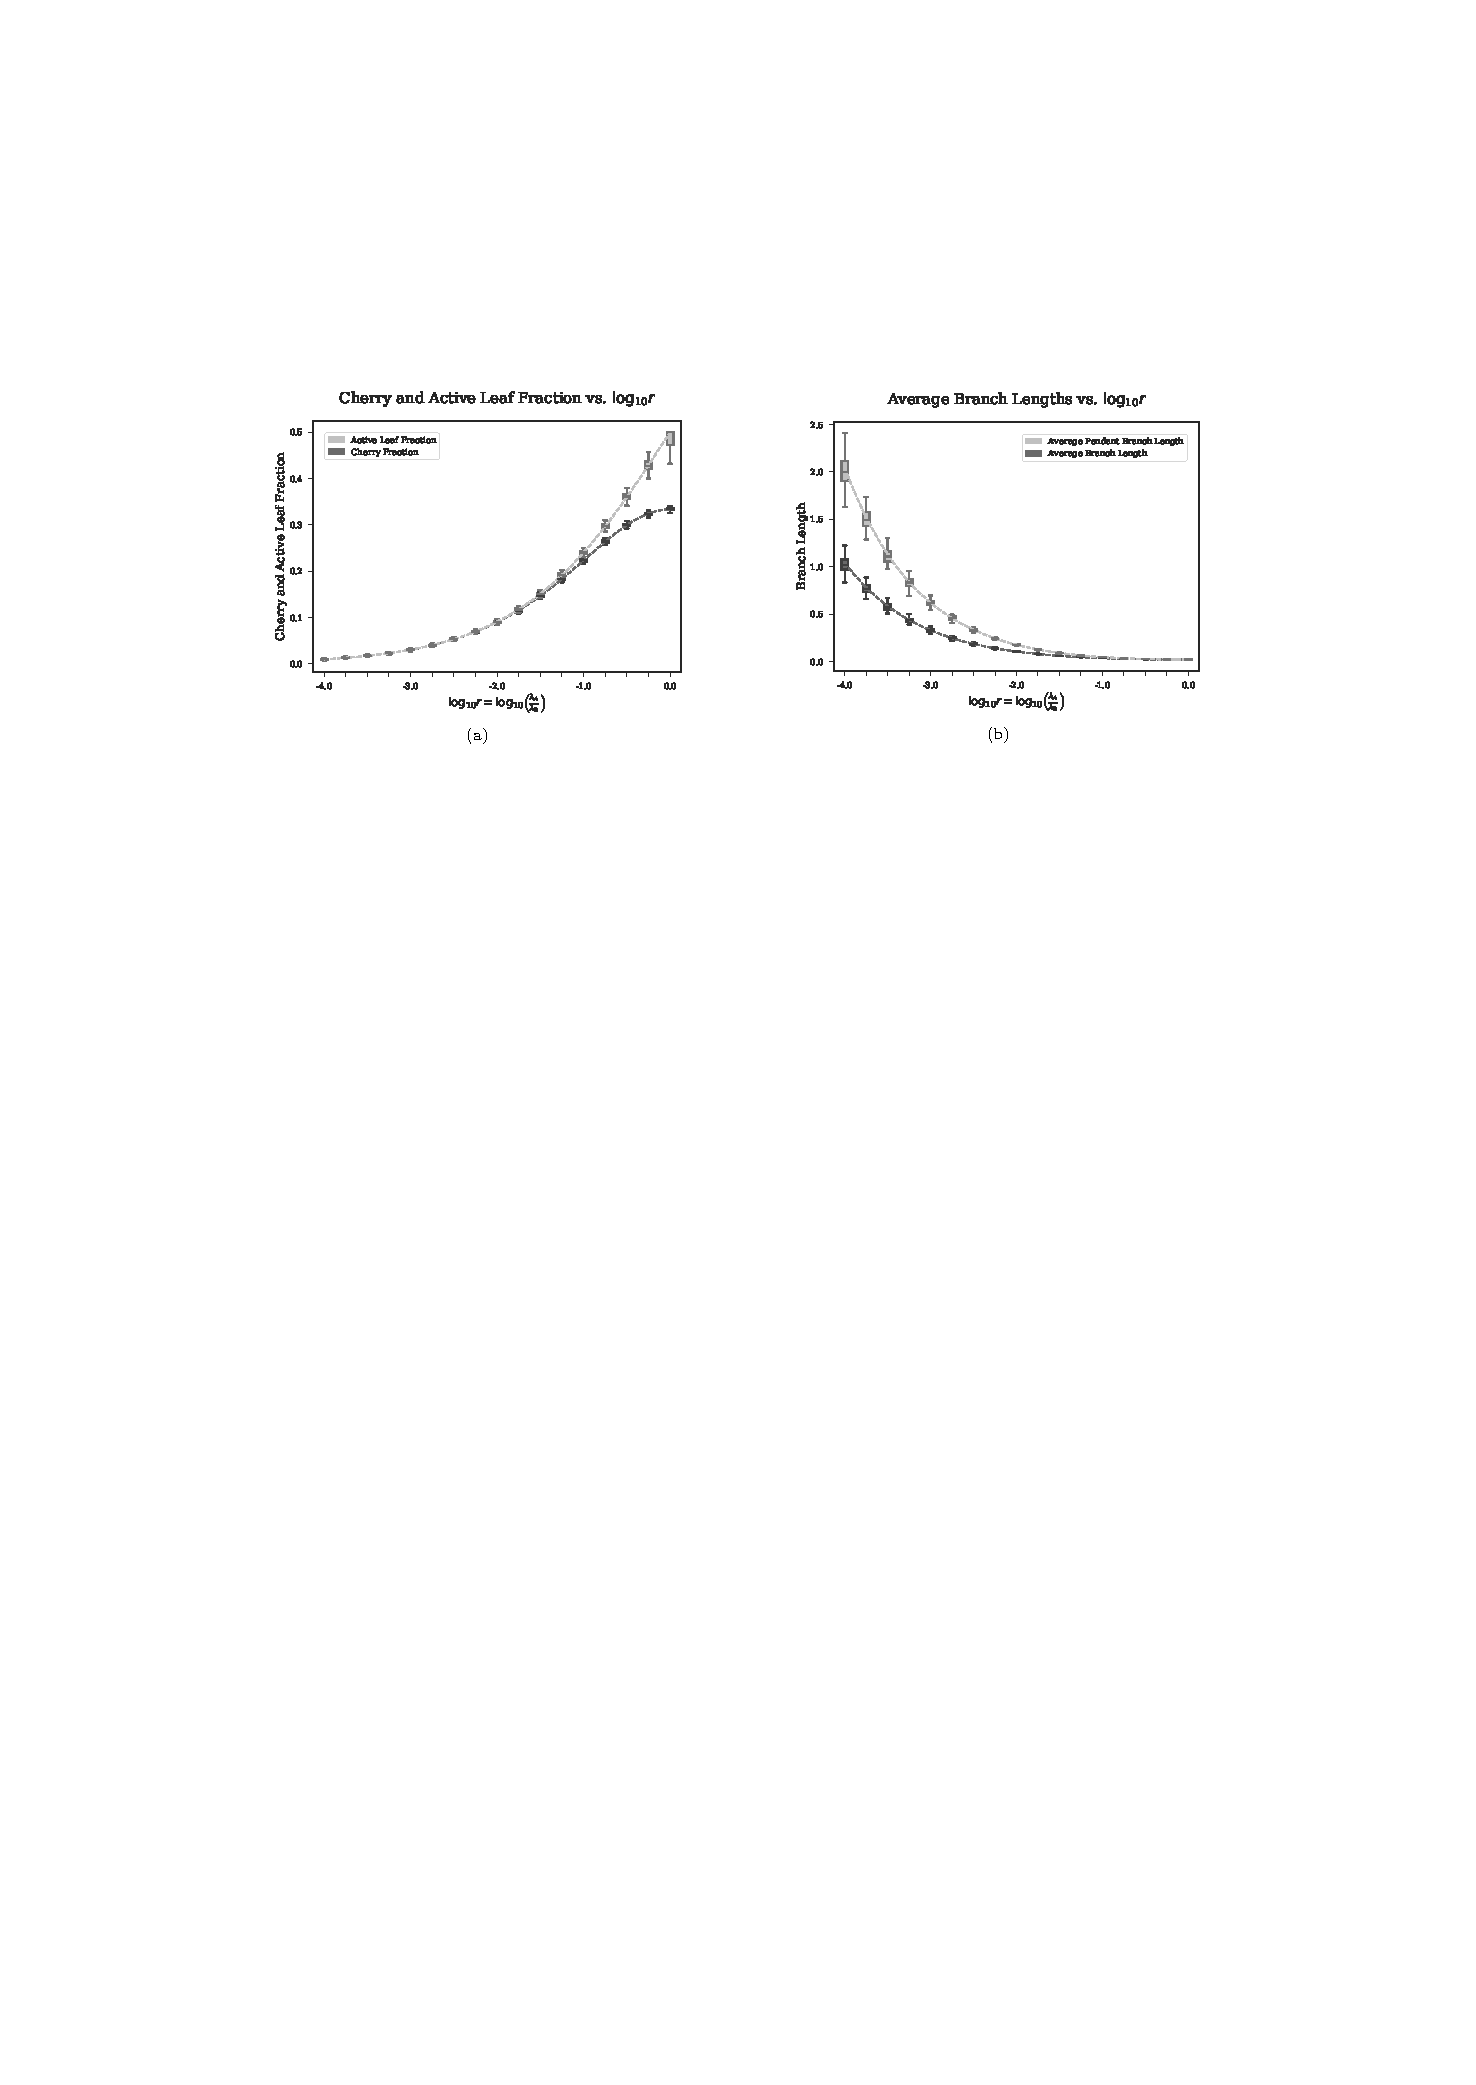
\includegraphics[width=\textwidth]{figs/dualbirth-c-vs-r}
\caption[Theoretical Expectations]
{Theoretical expectations of (a) cherry fraction (dashed dark gray line) and active leaf fraction (dashed light gray line), and (b) branch length (dashed dark gray line) and pendant branch length (dashed light gray line) versus simulated distributions (in box plots) using 100 replicates with $n=4096$, $\lambda=48$, and varying values of $r$ ($x$-axis) from $1/1024$ to $1$. Note that the number of cherries is the maximum parsimony estimate of the number of active elements, and the most parsimonious estimate works well for low values of $r$.}
\label{fig:dualbirth-c-vs-r}
\end{figure}

The proofs can be found in Section~\ref{sec:dualbirth-proofs}.
As Figure~\ref{fig:dualbirth-c-vs-r}a shows, these expectations closely match simulations results. As $r$ increases, the expected frequency of cherries increases until it reaches its peak at \sfrac{1}{3} for $r=1$. The number of active elements follows a similar pattern and reaches its peak at \sfrac{1}{2}  for $r=1$. Thus, under the Yule model, only half the nodes will be expected to be active (recall that an active element is defined as one that has already propagated). Also note $r=x$ and $r=\frac{1}{x}$ differ only in what elements are labeled left or right, and thus, they are indistinguishable for unordered trees. As noted before, $r>1$ does not have a meaningful interpretation in biological processes that we consider; thus, we focus on $0\leq r\leq1$.

\subsubsection{Expected Branch Length}
A natural quantity of interest under any model of tree evolution is the expected length of a random branch. For example, under the Yule model, branches are exponentially distributed with rate $1/2\lambda$~\cite{Mooers2012}. In our model, the expected branch length depends on both $\lambda$ and $r$. In all the results given below, we assume all the leaves are sampled. 
\begin{theorem}\label{thm:bl}
For a weighted tree shape $t$ generated by the dual-birth model with parameters $r$ and $\lambda$ conditioned on having $n$ leaves, let $\BL$ be an r.v.\ giving the length of a random branch in $t$; i.e., $\BL=\bl_I$ for $I\sim\mathcal{U}(1,n-2$). Then, 
\begin{align}\label{eq:bl}
\lim_{n\to\infty}\mathbb{E}(\BL) \to \frac{1}{2\lambda}\left(\frac{r+1}{\sqrt{r}}\right) = \frac{1}{\la}\frac{\sqrt{r}}{2}
\end{align}
\end{theorem}

The proof can be found in Section~\ref{sec:dualbirth-proofs}. For a fixed $\lambda$, increasing $r$ in $(0,1]$ reduces the expected branch lengths, resulting in the minimum value under the Yule model (Fig.~\ref{fig:dualbirth-c-vs-r}b).

\subsubsection{Expected Terminal Branch Length}
Under the Yule model, terminal and internal branch lengths have the same expected length~\cite{Mooers2012}. For $r\ll1$, we expect that inactive entities result in long terminal branches and relatively short internal branches. These expectations can be confirmed in simulations. As expected, close to $r=1$, the mean terminal branch length is close to the mean branch length but the two values gradually diverge as $r$ decreases (Fig.~\ref{fig:dualbirth-c-vs-r}b). Therefore, the difference between average terminal and internal branch lengths is a function of $r$, and therefore, a closed-form formula for the expected terminal branch length would be useful in building an estimator of $r$. While we don't have a proven result for the terminal branch length, based on simulations, we present a conjecture. Note that this conjecture was purely reached based on our intuition and trial-and-error, starting from Equation~\ref{eq:bl} and modifying the denominator until a close match to the empirical values was obtained.

\begin{conjecture}\label{thm:tbl}
For a weighted tree shape $t$ generated by the dual-birth model with parameters $r$ and $\lambda$ conditioned on having $n$ leaves, let $\TBL$ be an r.v.\ giving the length of a random terminal branch in $t$. Then, 
\begin{align}\label{eq:tbl}
\lim_{n\to\infty}\mathbb{E}(\TBL)\to\frac{1}{\la}\left(\frac{\sqrt{r}}{1+2\sqrt{r}-r}\right)
\end{align}
\end{conjecture}

Figure~\ref{fig:dualbirth-c-vs-r}b shows that the conjectured results closely match the observed mean terminal branches for a wide range of $r$ values. Note that changing $\la$ simply scales all lengths, so our simple simulations have explored \textit{all} free parameters of the dual-birth model (albeit, only for $r\in[10^{-4},1]$ range). Regardless of whether our conjecture is true (which cannot be proven by simulations), the close match of Equation~\ref{eq:tbl} and simulated results means that we can use it to provide an approximate estimator of $r$.

\subsubsection{Parameter Estimation}\label{sec:dualbirth-paramest}
Theorem~\ref{thm:cherr} enables us to estimate the $r$ parameter for a given tree. Given a tree with $c$ cherries, and for $x=c/n$, solving for $r$ in Equation~\ref{eq:cherries} results in the following relationship (Fig.~\ref{fig:dualbirth-sup-cvsr}):
\begin{equation}\label{eq:rforc}
\hat{r}(x)=\bigg(\frac{1-x-\sqrt{(x+1)(1-3x)}}{2x}\bigg)^2
\end{equation}
for $x\leq \frac{1}{3}$ and else $\hat{r}(x)=1$.

An alternative estimator can be designed by combining Theorem~\ref{thm:bl} and Conjecture~\ref{thm:tbl} for expected total and terminal branch length. Given a tree with an average branch length of $d$ and an average terminal branch length of $l$, solving Equations~\ref{eq:bl}~and~\ref{eq:tbl} for $r$ and $\lambda_a$, we can design the following estimator for large $n$:
\begin{equation}\label{eq:rforbl}
\hat{r}(b,l) = \left(1-\sqrt{2\left(1-\frac{d}{l}\right)}\right)^2
\end{equation}

Further approximating the total average branch length to be the mean of internal branch lengths ($i$) and terminal branch lengths (a good approximation for large $n$), we can further simplify Equation~\ref{eq:rforbl} to:
\begin{equation}\label{eq:rforbl-approx}
\hat{r}(i,l) = \left(1-\sqrt{1-\frac{i}{l}}\right)^2
\end{equation}

Having estimated $r$, we can easily use Equation~\ref{eq:bl} to get an estimate of $\lambda$ from the observed mean branch length for large $n$. Note that, absent a proof for Conjecture~\ref{thm:tbl}, Equation~\ref{eq:rforbl} should be treated as an approximate estimator. Also note that this approximate estimator assumes the given tree itself was generated by the dual-birth model (e.g. it is not the result of subsampling the tips of a tree generated by the dual-birth model). We discuss statistical properties of both estimators in Section~\ref{sec:dualbirth-estimator-properties}.

\subsubsection{Sampling the Dual-Birth Model}\label{sec:samplingalgo}\label{sec:db-algo}
When conditioning on $n$, the number of tips, a simple algorithm can be used to sample the space of ordered weighted tree shapes defined by the dual-birth model.

We start with a single-node tree and iteratively add new nodes until the tree has $n$ leaves. We use a heap to keep a list of current leaves sorted by their distance to the root. In each iteration, we add two child nodes to the highest leaf in the tree (i.e., the leaf closest to the root); we sample from two exponential distributions with rates $\la$ and $\lb$ for the left and right child's branch lengths, respectively. The two new nodes are added to the heap of leaves, and the parent is removed from the heap. Once the loop has terminated, we truncate the tree by shrinking all terminal edges except the one attached to the leaf that is closest to the root such that all leaves are equidistant to the root.

%\paragraph{Correctness:}
Hartmann \textit{et al}. have described various strategies for sampling trees with $n$ leaves~\cite{Hartmann2010}. Our sampling procedure falls under what they have termed \gls{SSA}. As they point out, the \gls{SSA} procedure produces the right distribution on tree topologies for pure birth models, like ours, because, once the process reaches $n$ tips for the first time, it never goes back to having fewer tips. A remaining question is what distribution should be used to decide the time between when $n$ leaves first become present until we stop the simulation (call it $\tav$). Let $h(\tav)$ be the p.d.f of that waiting time. If the time between when we have $n$ leaves and the the birth of leaf $n+1$ is given by $x>\tav$, then $\tav$ should be uniformly sampled between zero and $x$. Moreover, the probability of sampling each tree with $n$ leaves should be proportional to $x$, the time it remains an $n$-leaf tree. Thus, as Hartmann \textit{et al}.show, by summing over all possible values of $x$, we get:
\begin{small}
\begin{eqnarray}\label{eq:h}
h(\tav) \propto \int_{x=\tav}^{\infty} x.h(\tav|x).g_{n-1}(x) \ \mathrm{d}x &=& \int_{x=\tav}^{\infty} x.\frac{1}{x}.g_{n-1}(x) \ \mathrm{d}x  \nonumber \\ 
&=& \int_{x=\tav}^{\infty} g_{n-1}(x) \ \mathrm{d}x
\end{eqnarray}
\end{small}
where $g_{n-1}$ is the p.d.f of a random variable (r.v.) for $x$. In our model, this r.v.\ is equivalent to the minimum of $n$ exponential r.v.s, $\LB{n-1}$ of which have rate $\la$ and the rest have rate $\lb$; thus, $g(x)$ is the p.d.f of an exponential with rate $\lambda_{n-1}=\lambda_a \LB{n-1}+\lambda_b(n-\LB{n-1})$. It is easy to see that Equation~\ref{eq:h} simplifies to $h(\tav)\propto g_{n-1}(\tav)$. Thus, the correct waiting time between the last birth event and the end of the simulation is identical to the waiting time for the birth event that would create $n+1$ leaves.

Note that, if we were conditioning on $\tau$ (the tree height) instead of $n$, the same procedure would remain correct, except we would continue until all leaves have at least the required height and would then cut branches that are longer than $\tau$.

\subsection{Simulation Setup}
\subsubsection{Datasets}
Given a set of parameters, we use our implementation of the fixed-$n$ sampling procedure  to generate 20 replicate ``true'' trees. We then deviate each tree from ultrametricity by multiplying each branch of the tree by a multiplier sampled from a gamma distribution with shape and rate both set to $\alpha$ (with an expected value of 1). For each true tree, we then use INDELible~\cite{Fletcher2009} and the \gls{GTR}+$\Gamma$ model~\cite{Tavare1986} to simulate a multiple sequence alignment with no indels, which is later used to infer the tree. The simulation parameters are \textit{n}, $r$, $\lambda$, and deviation from ultrametricity (i.e., the shape of the Gamma distribution, $\alpha$). For sequence evolution, the parameters to select are $k$ (the sequence length), the \gls{GTR} parameters, and the Gamma rate across sites. We also vary model of sequence evolution used for inference.

\begin{table}[!ht] % TABLE 1 IN ORIGINAL PAPER
\caption[Experiments]{Experiments (default parameters in bold)}
\vspace{-0.25in}
\begin{center}
\begin{tabular}{|l|l|l|}
\hline
{\bf\#}&{\bf Parameter} & {\bf Parameter Values}\\
\hline
1&$r$ (const. bl) & $10^{-4}, 10^{-3}, {\bf 10^{-2}}, 10^{-1}, 10^{0}$\\
2& Model & JC69, K80, HKY85, GTRCAT, \textbf{GTR+$\Gamma$}\\
3&$\lambda$ & $33.866, 84.664, {\bf 169.328}, 338.655, 846.64$\\
4&$k$ & $50, 100, 200, {\bf 300}, 600, 1200, 2400, 4800$\\
5&$n$ & $25, 50, 250, 500, {\bf 1000}, 2000, 4000$\\
6& $\alpha$ (clock) & $2.952, 5.904, {\bf 29.518}, 147.591, 295.182, \infty$\\
\hline
\end{tabular}
\end{center}
\label{tab:dualbirth-experiments}
\end{table}

We perform six \textit{experiments}, each varying a single parameter (Table~\ref{tab:dualbirth-experiments}). The exception is $r$, for which we modify both $r$ and $\lambda$ to keep expected branch length constant. Each experiment is centered around a default set of parameters chosen to emulate our \textit{Alu} dataset (details in Section~\ref{sup:simsetup-mot}).

\subsubsection{Methods}
We infer trees from the simulated sequence data using FastTree-II~\cite{Price2010} and RAxML~\cite{Stamatakis2014}. We estimate $r$ using the cherry-based (Eq.~\ref{eq:rforc}) and length-based (Eq.~\ref{eq:rforbl}) estimators.

\subsubsection{Error Measurement}
We measure the accuracy of inferred tree topologies using the normalized \gls{RF} distance~\cite{Robinson1981}, which is equal to the proportion of the branches that are different between the true and inferred trees. To account for the sensitivity of \gls{RF} distance to rogue tips, especially for caterpillar trees, we also compute the \gls{MS} metric, implemented in TreeCmp~\cite{Bogdanowicz2012}. We compute differences between the log-likelihood scores of true and inferred trees using RAxML. To measure the accuracy of our estimates of $\lambda$ and $r$, we compute the log-ratio of true versus inferred values for both parameters and show the resulting distribution.

\subsection{Human \textit{Alu} Dataset}
Most analyses of \textit{Alu} elements have relied upon the classification of elements into subfamilies and using consensus sequences. Because the subfamily classification is potentially incomplete~\cite{Price2004}, we analyze a large dataset of 885,011 \textit{Alu} repeats.

\subsubsection{Data Acquisition}\label{sec:aluseqs}
We use the Dfam database~\cite{Hubley2016} to search for \textit{Alu} repeats. We first create a database containing only Human \textit{Alu} profile \glspl{HMM} from Dfam. We then use nhmmer (via Dfam's \texttt{dfamscan.pl} script) to scan the hg19 reference genome using this subset of Dfam. nhmmer computes a bitscore for each result, which is a metric of how well the sequence matches its respective profile HMM in comparison to how well a random sequence would match the same model. Our motivation to use Dfam profile \glspl{HMM} to scan for \textit{Alu} sequences is their sensitivity to detect sequences with deviation from the subfamily consensus, but this same sensitivity also allows for false hits. To combat this, for each \textit{Alu} subfamily, we filter out all sequences with low bitscores. We use unique bitscore thresholds for each \textit{Alu} subfamily because of the heterogeneity of bitscore distributions across subfamilies (see Figs.~\ref{fig:dualbirth-bit-hists}~and~\ref{fig:dualbirth-bit-thresh} for our choices of thresholds).

\subsubsection{Alignment and Tree Inference}\label{sec:alutree}
We estimated a \gls{MSA} on the set of 936,664 bitscore-filtered \textit{Alu} sequences using\break PASTA~\cite{Mirarab2015}. Some of the sequences in the resulting MSA were short (Fig.~\ref{fig:dualbirth-non-gap-hist}), which could negatively impact tree inference. To combat this potential risk, we filtered out any sequences that had less than 200 non-gap characters in the \gls{MSA}. Our final dataset contained 885,011 full-length \textit{Alu} sequences. Our \gls{MSA} included some extremely gappy sites, as is expected for any dataset including these many sequences. We masked all sites in the PASTA alignment where 99\% or more of characters were gaps. Prior to masking, there was a total of 266,699,287 non-gap characters in the \gls{MSA}; masking reduced the number to 264,144,814 non-gap characters in the \gls{MSA} (99.04\% retention). Since gaps are treated as missing data in our tree inference methods (and not as phylogenetically informative indels), the removal of 1\% of the data should result in minimal loss of phylogenetic information. The consensus sequence of the final alignment (Fig.~\ref{fig:dualbirth-alu-tree}a) included many conserved sites. We used FastTree~2~\cite{Price2010} to infer a tree on the masked alignment under the \gls{GTR}+$\Gamma$ model. The resulting tree was not well-supported (Fig.~\ref{fig:dualbirth-support-vals}), a fact that is not surprising considering the short sequence length and low divergence. We also used RAxML~\cite{Stamatakis2014} to infer a tree on the masked alignment under the \gls{GTR}+CAT model. Our attempts to infer a tree under the \gls{GTR}+$\Gamma$ model using RAxML were unsuccessful.

Finally, to test the stability of our estimates, we performed a series of subsampling experiments in which we performed 20 subsampling replicates for $n$ = 1,000, 10,000, and 100,000 sequences, inferred trees using FastTree~2, and estimated parameters from those trees just as before.

\section{Results}
\subsection{Simulations: Dual-Birth Model}
We study the effects of parameters on tree reconstruction accuracy and the ability to estimate $r$.

\subsubsection{Tree Accuracy}
The topological tree accuracy was heavily influenced by $r$, $\lambda$, and sequence length (Fig.~\ref{fig:dualbirth-tree-inference-error}a). Shortening branch lengths (by increasing $\lambda$) increased the error (Fig.~\ref{fig:dualbirth-tree-inference-error}a, upper-right) as expected. Reassuringly, increasing sequence length reduced the error; while with the default 300 sites, the topological error was 38\%, the  error reduced to 6\% with 4,800 sites (Fig.~\ref{fig:dualbirth-tree-inference-error}a, lower-left).

\begin{figure} % FIGURE 3 IN ORIGINAL PAPER
\centering
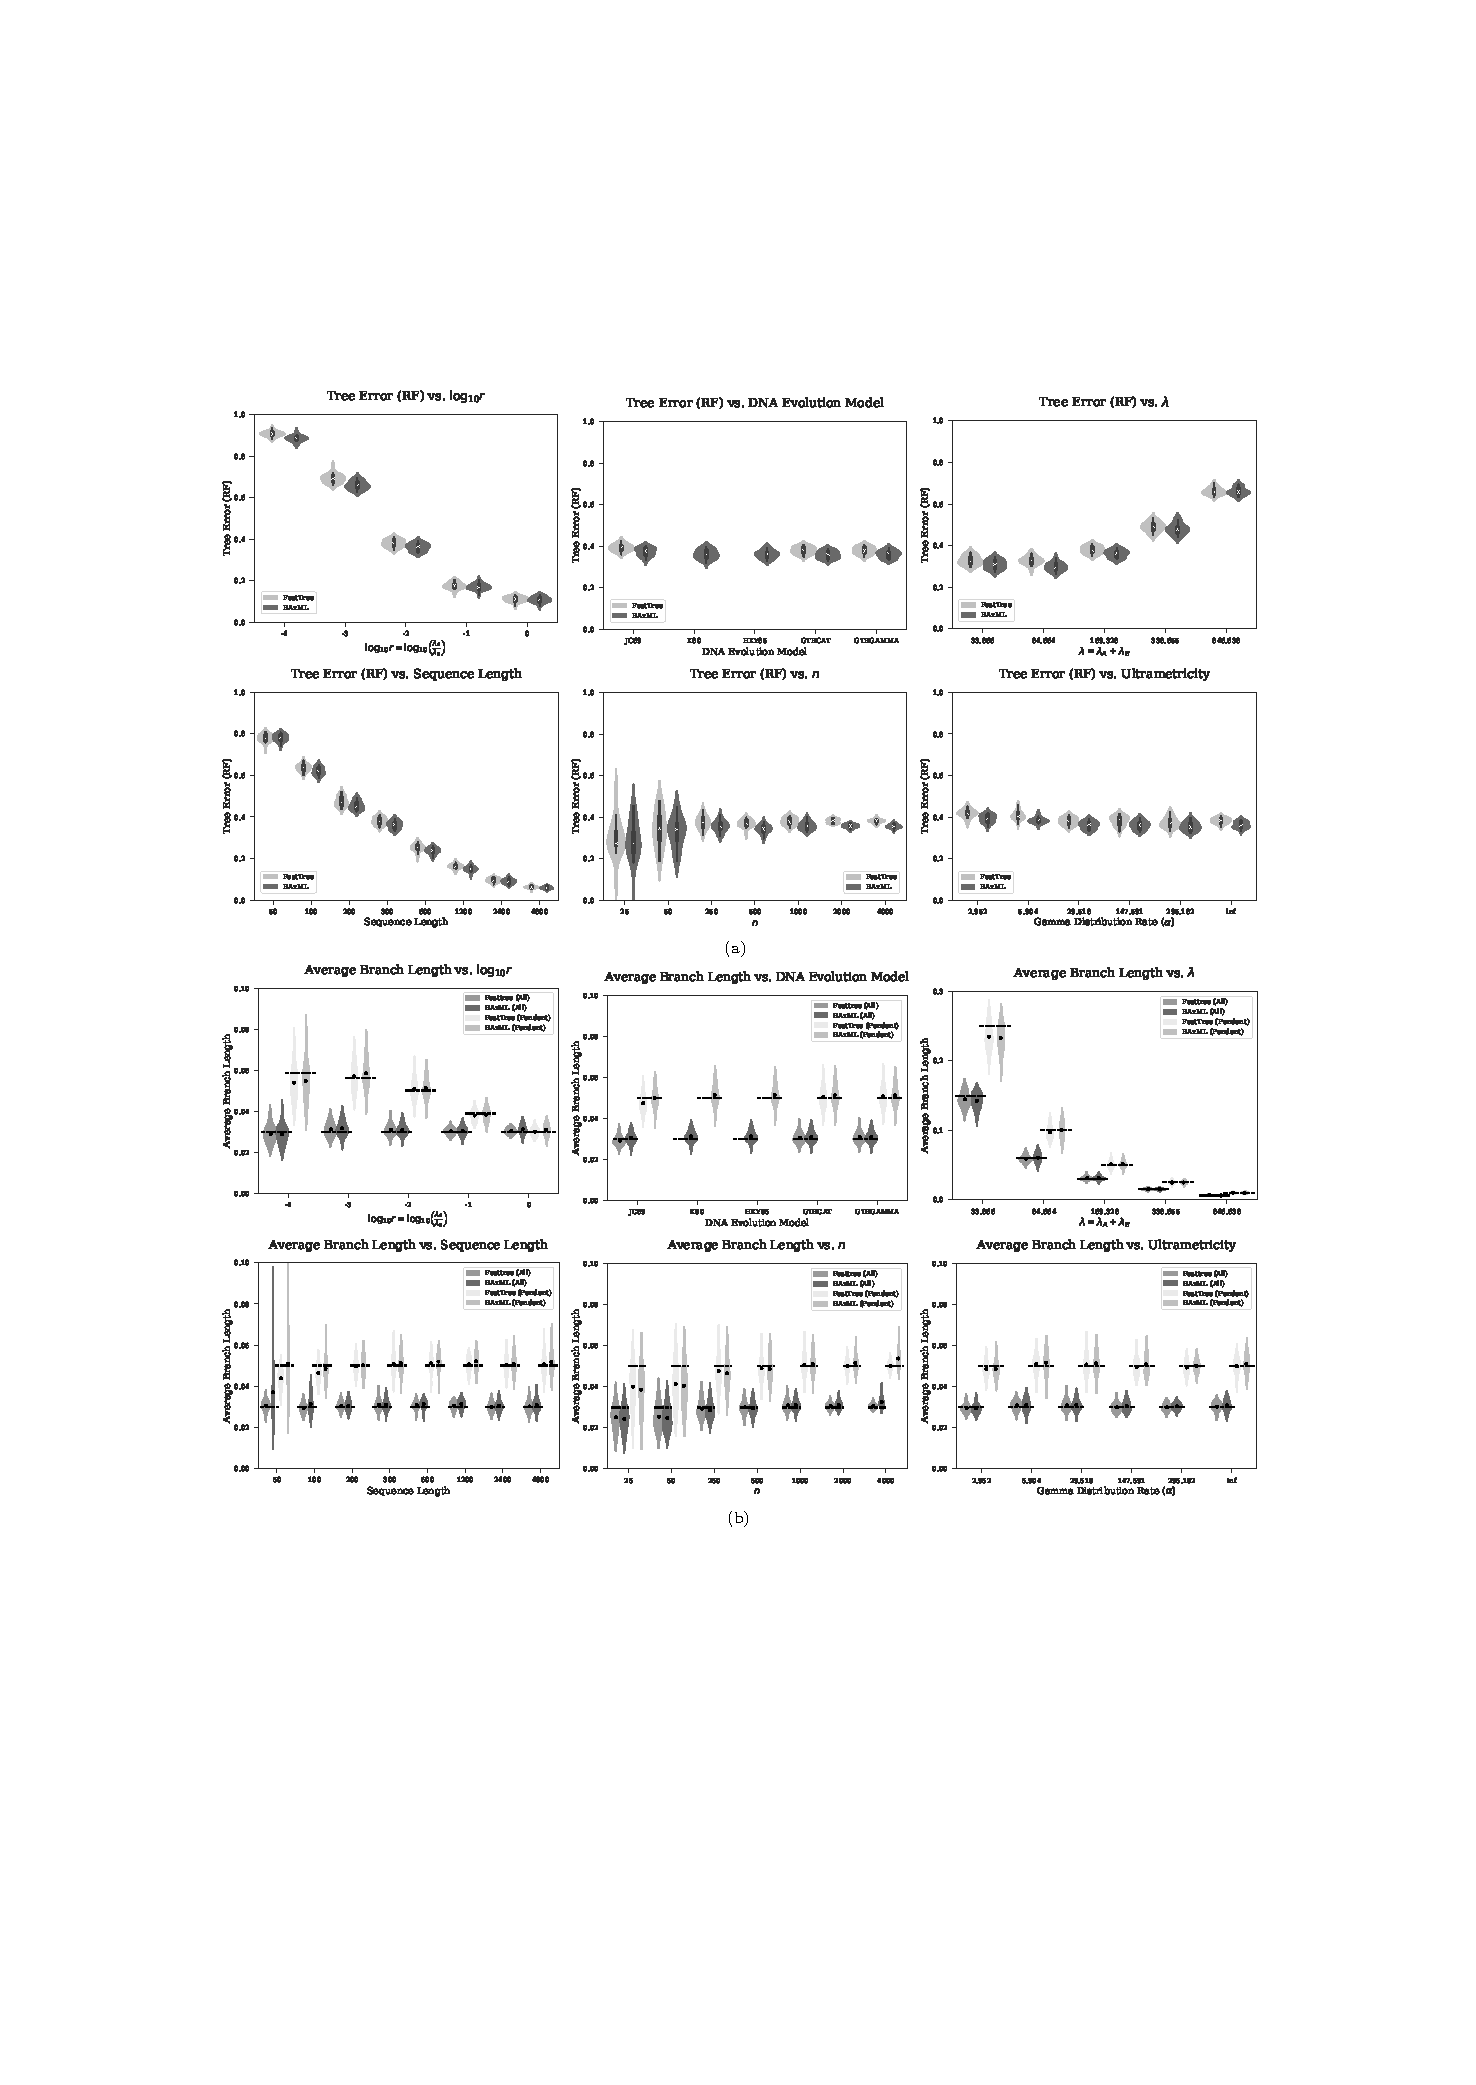
\includegraphics[width=\textwidth]{figs/dualbirth-tree-inference-error}
\caption[Tree Inference Error]
{Tree inference error. Violin plots are shown for (a) the \gls{RF} distance between true and estimated trees, and (b) mean branch lengths and mean pendant branch lengths computed for each tree (the dashed lines show the theoretical and conjectured expectations, and the dots show empirical averages). Note that FastTree~2 does not implement the \gls{K80} and \gls{HKY85} models.}
\label{fig:dualbirth-tree-inference-error}
\end{figure}

Most interestingly, the topological error depended on the parameter $r$ (Fig.~\ref{fig:dualbirth-tree-inference-error}a, upper-left). When $r=1$ (i.e., the Yule model), tree estimation error was relatively low. As we reduced $r$, which progressively made the true trees less balanced, the topological error quickly increased (Fig.~\ref{fig:dualbirth-tree-inference-error}a, upper-left). With $r=10^{-4}$, where the tree is almost fully unbalanced, the \gls{RF} error ranged between 85\% and 94\%. Similar patterns were observed when we used the \gls{MS}~\cite{Bogdanowicz2012} measure of error (Fig.~\ref{fig:dualbirth-tree-ms}). These extremely high levels of error for unbalanced trees are interesting considering the fact that the sequence length and the expected branch length are kept fixed.

Interestingly, the number of leaves, $n$, mostly affected the variance of the topological error. As $n$ increases, the average tree error remained relatively constant, but its variance gradually reduced (Fig.~\ref{fig:dualbirth-tree-inference-error}a, lower-center). Deviations from the clock had very small impact on the topological tree accuracy (Fig.~\ref{fig:dualbirth-tree-inference-error}a, lower-right). The choice of the sequence evolution model similarly had minimal impact on accuracy (Fig.~\ref{fig:dualbirth-tree-inference-error}a, upper-center). Note that the \gls{GTR}+$\Gamma$ model was used for simulation (with parameters given in the supplement); thus, all other results include model misspecification.

To make sure the difficulty in correctly resolving unbalanced trees is not simply due to insufficient search in ML tools, we compared likelihood scores of inferred trees and their corresponding true trees (Fig.~\ref{fig:dualbirth-tree-score-diff}). Two interesting patterns were observed. The RAxML tree consistently had better scores than the true tree, indicating that lack of accuracy was not simply due to insufficient search. The difference in log-likelihood scores narrowed as $r$ increased. These patterns are consistent with the explanation that likelihood scores computed on limited data are progressively less predictive of tree accuracy as the trees become less balanced. It is well-known that trees that include a mix of long and short branches, or generally, high heterogeneity of branch length, are hard to estimate, even in a likelihood framework~\cite{Kuhner1994,Kolaczkowski2004}. Decreasing $r$ increased branch length heterogeneity in our dataset (Fig.~\ref{fig:dualbirth-tree-bl-supp}); the increased heterogeneity may be a cause of the large number of sites required for accurate estimation using maximum likelihood. 

Unlike tree topology, the estimated average branch length and average terminal branch length were relatively accurate and robust to the parameters choice (Fig.~\ref{fig:dualbirth-tree-inference-error}b). However, two interesting and related patterns should be noticed. For $r=10^{-4}$, both the terminal and overall branch lengths had slightly lower empirical means compared to the theoretical results or the conjecture (Fig.~\ref{fig:dualbirth-tree-inference-error}b, upper-left). This may partially be due to the fact that our theoretical results/conjectures are asymptotic in $n$, so the estimators may be biased for limited $n$. Consistent with this explanation, we observed that for $r=10^{-2}$, with small $n$, empirical branch length averages were consistently lower than the theoretical values, but that they gradually increased and reached the theoretical expectations around $n=500$ (Fig.~\ref{fig:dualbirth-tree-inference-error}b, lower-center). The required $n$ for the asymptotic expectations to be accurate will likely depend on $r$, and $r$ values in the $10^{-4}$ range likely require $n>1000$.

Overall, RAxML consistently outperformed FastTree~2 with respect to tree accuracy by a small margin.

\begin{figure} % FIGURE 4 IN ORIGINAL PAPER
\centering
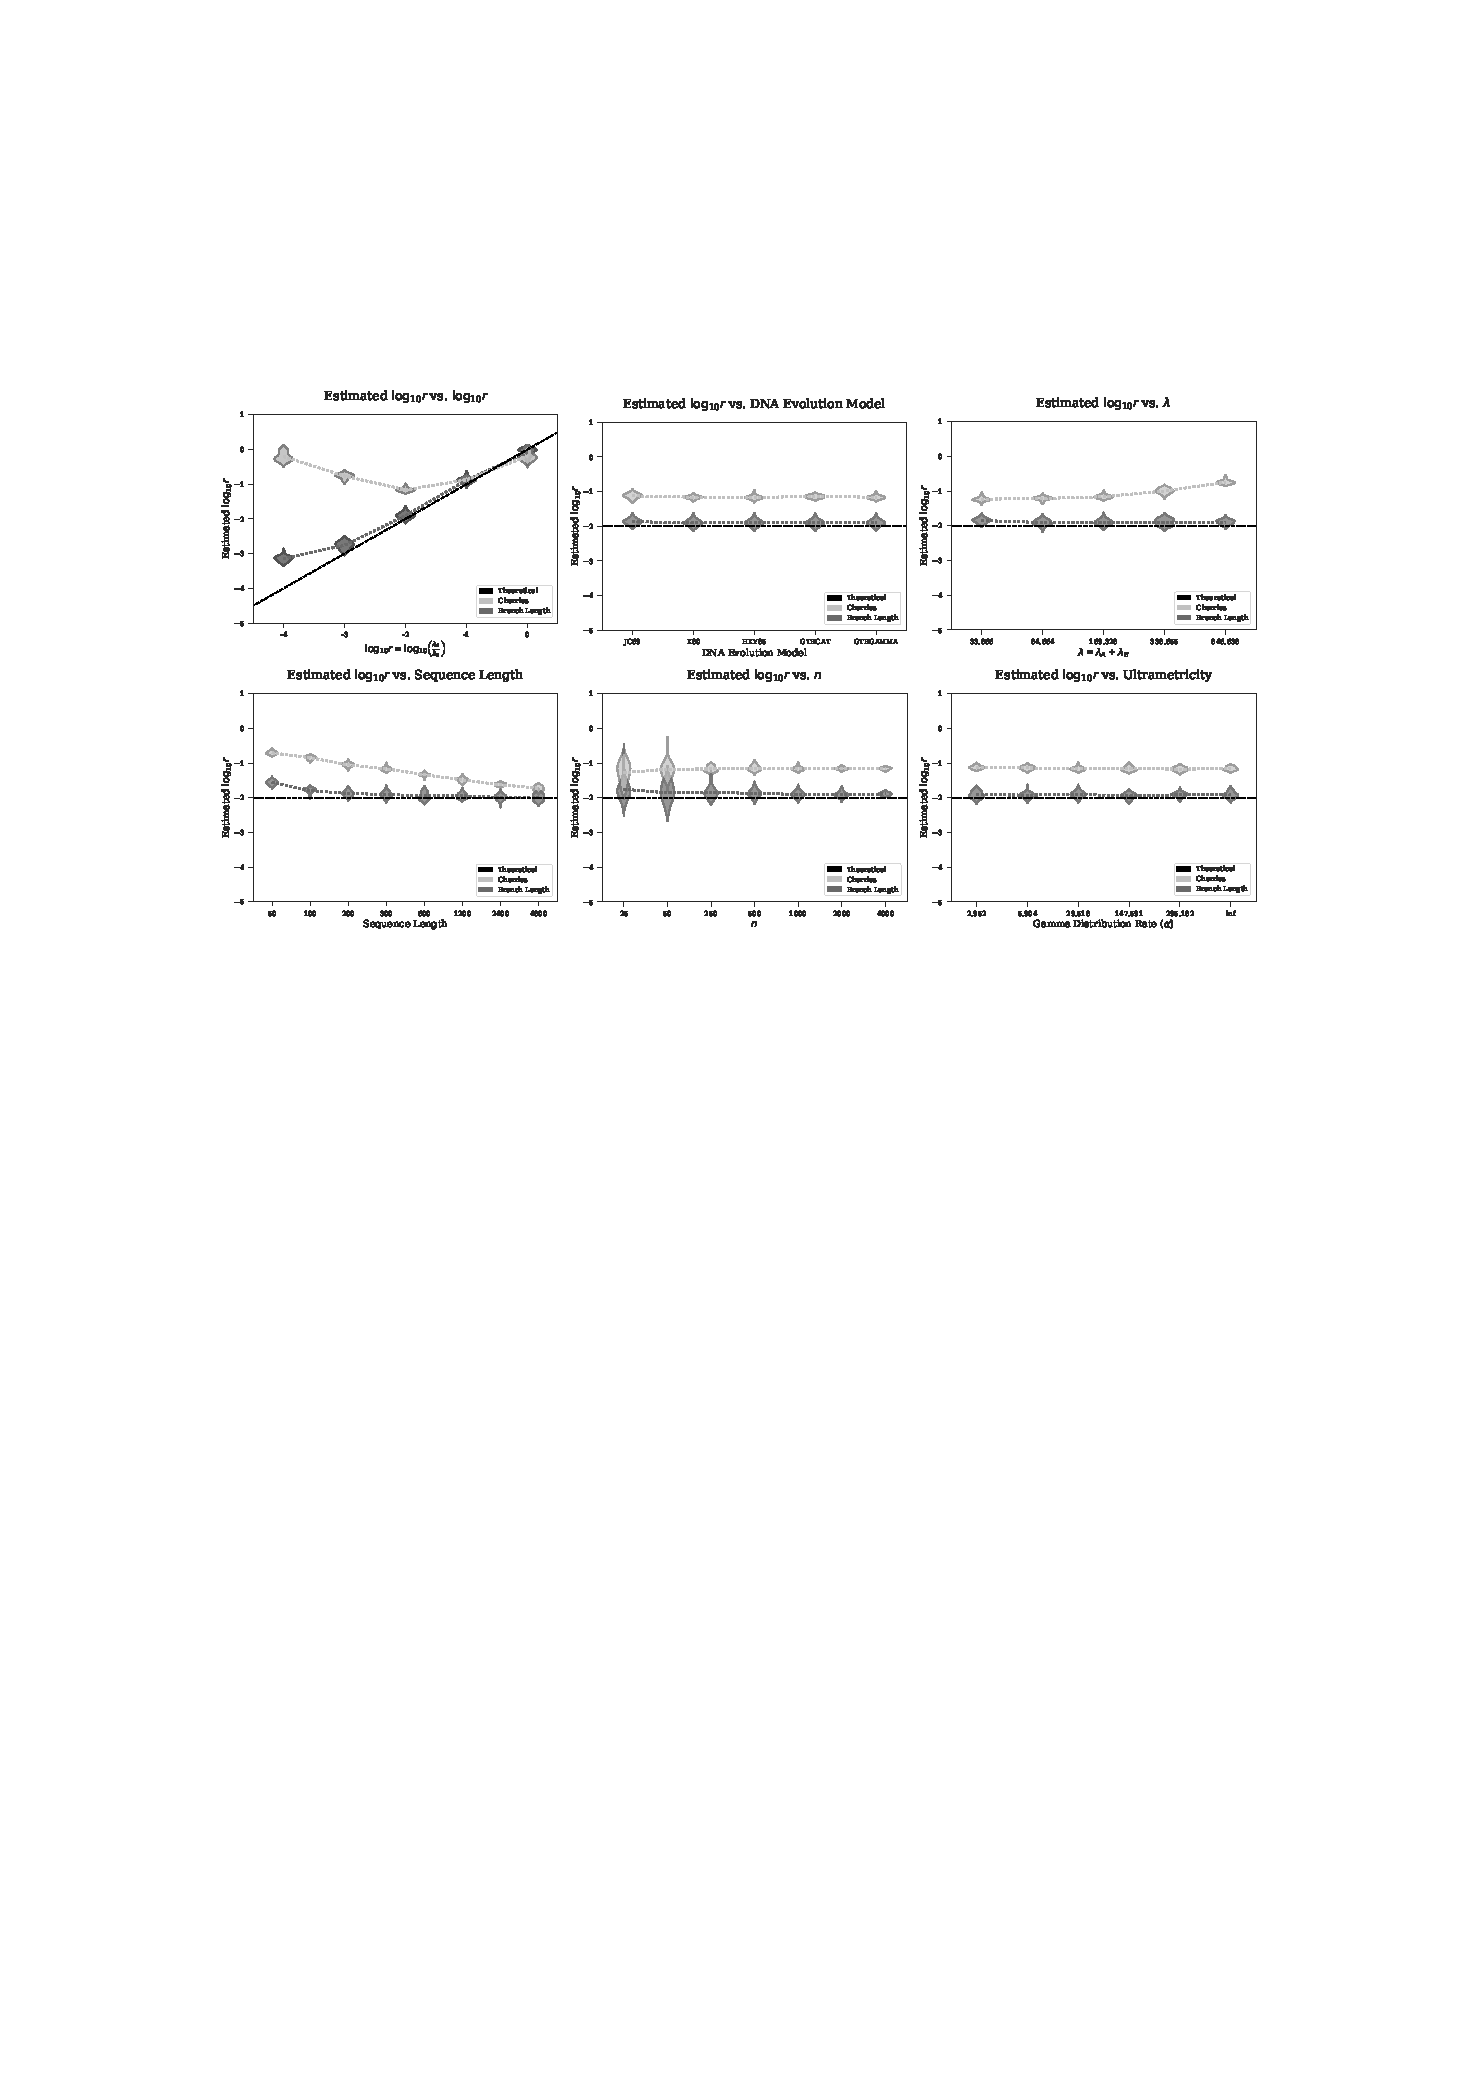
\includegraphics[width=\textwidth]{figs/dualbirth-param-est-accuracy}
\caption[Parameter Estimation Accuracy]
{Parameter estimation accuracy. Violin plots are shown for the estimated $r$, using the cherry-based estimator and the branch-length-based estimator, for each of the experiments. True values are shown as dashed black lines.}
\label{fig:dualbirth-param-est-accuracy}
\end{figure}

\subsubsection{Accuracy of $\hat{r}$}\label{accuracy-cherries}
We focus on RAxML trees here, but note that FastTree trees give similar results (Fig.~\ref{fig:dualbirth-res-cherry-supp}).

We start with the cherry-based $r$ estimator. Unlike estimates based on true trees that were highly accurate (Fig.~\ref{fig:dualbirth-res-cherry-supp}), when trees inferred from sequence data are used, the cherry-based estimator is often not accurate (Fig.~\ref{fig:dualbirth-param-est-accuracy}). When $r=1$, estimates from cherry fraction are close to true values. However, for small $r$, the cherry fraction can be dramatically overestimated (Fig.~\ref{fig:dualbirth-cherry-fraction-supp}), and as a result, the estimated $r$ can be orders of magnitude larger than the true value (Fig.~\ref{fig:dualbirth-param-est-accuracy}). For example, when the true value of $r$ is $10^{-4}$, RAxML inferred around 30\% cherry fraction (i.e., $\hat{r}\approx 1$) instead of 0.99\% (Fig.~\ref{fig:dualbirth-cherry-fraction-supp}). Since on true trees the estimator works very well (Fig.~\ref{fig:dualbirth-res-cherry-supp}), the overestimation is clearly due to tree inference error. Consistent with this explanation, as the length of the sequence increases, the cherry fraction and $\hat{r}$ gradually converge to the true values; with 4,800 sites, the estimated $r$ is within 27\% of the true value (Fig.~\ref{fig:dualbirth-param-est-accuracy}, bottom-left).

Unlike the cherry-based estimates, the length-based estimates of $r$ were generally
quite accurate (Fig.~\ref{fig:dualbirth-param-est-accuracy}).
While the estimator showed patterns that indicated it may be biased, it gave reasonable estimates of $r$ for most conditions. The length-based method tended to slightly overestimate $r$ in most conditions, but the overestimation was substantial only for $r=10^{-4}$; even for this most difficult case, however, estimates were still  within one order of magnitude from the true value. Also, when sequences were extremely short (50 \gls{bp}), $r$ was substantially overestimated but was still within an order of magnitude of the true $r$. Even though the estimator is based on asymptotic results on $n$, reducing $n$ to small values still maintained relatively high accuracy; only at $n\leq 50$ did the variance of the estimator start to increase such that distributions of the estimate spanned more than an order of magnitude. Overall, the estimates are in the correct order of magnitude for most conditions, and are especially accurate for $10^{-3}\leq r\leq1$ for $k=300$, and this range is even wider for larger $k$.

\subsection{Simulations: Model Violations}
Our results so far were based on trees that completely followed the dual-birth model (save for the enforced divergences from the ultrametricity). We now explore the performance under conditions in which the  model generating the true tree diverges from our model. Specifically, we explore the following model: instead of forcing each node to have one child with rate $\la$ and another with rate $\lb$, with some small probability $p$, we allow both children to be active right away and thus have the rate $\lb$. Setting $p=0$ recaptures the dual-birth model, but increasing $p$ gradually introduces more model violations; $p=1$ simply gives the Yule model.

\begin{figure} % FIGURE 5 IN ORIGINAL PAPER
\centering
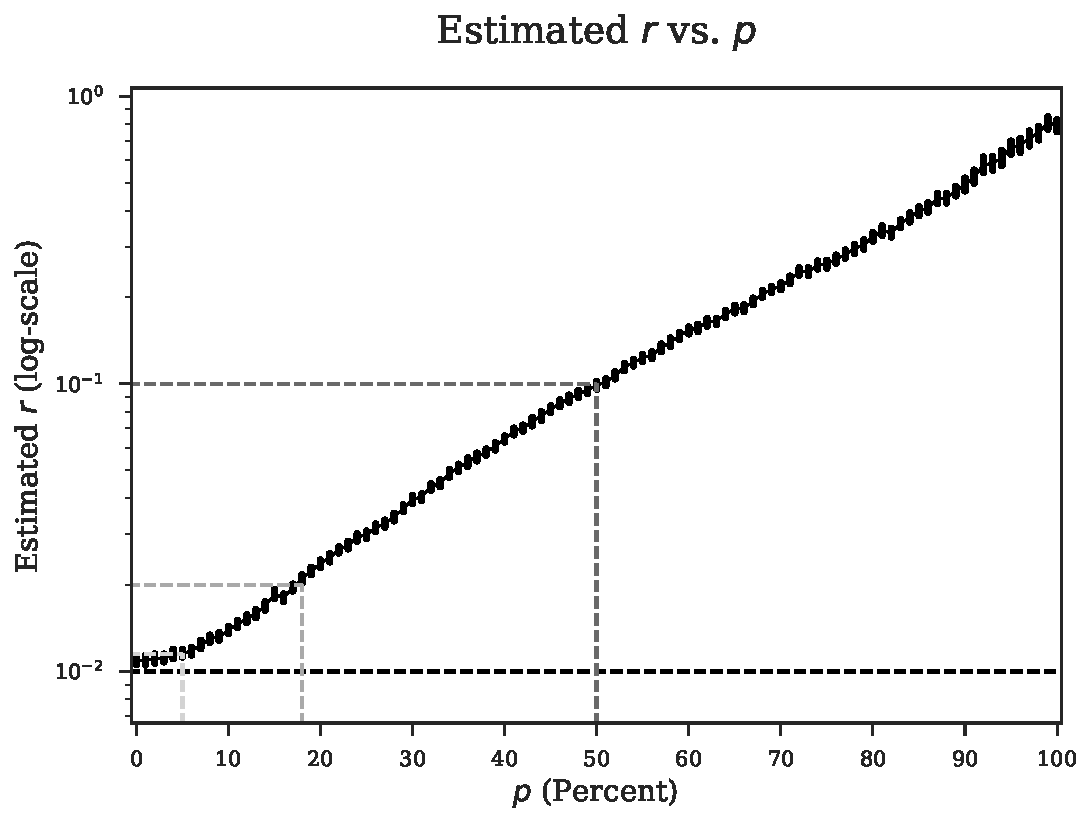
\includegraphics[width=0.7\textwidth]{figs/dualbirth-model-violations}
\caption[Model Violations]
{Model violations. Length-based estimates of $r$ vs. $p$, the probability that both children of a given branch are active (i.e., have rate $\lb$) based on 20 replicates of simulations per $p\in[0,1]$ with $n=1000$, $r=10^{-2}$, $\lambda=169.328$. Dashed light gray line: $p=0.05$; dashed medium gray line: $\hat{r}=2\times r$; dashed dark gray line: $\hat{r}=10\times r$.}
\label{fig:dualbirth-model-violations}
\end{figure}

We performed simulations in which we used the default experiment parameters (Table~\ref{tab:dualbirth-experiments}) but varied $p$ from 0 to 1. As expected, the error in $\hat{r}$ increases as $p$ approaches 1 (Fig.~\ref{fig:dualbirth-model-violations}). The length-based estimator was  robust to relatively low levels of model violation. For example, with $p=0.05$, the average estimated $r$ was $0.0116$, which is very close to the true value of $0.01$. Further increasing $p$ up to $0.17$, the average estimate of $r$ remained within two times the true value; errors reached an order of magnitude only at $p=\frac{1}{2}$. Interestingly, in log-scale, there was a somewhat linear relationship between $p$ and $\hat{r}$.

\subsection{Human Alu Analysis}\label{sec:dualbirth-human-alu-analyses}
We study two questions: How many {\em Alu} elements are active? At what rates do inactive {\em Alu} elements become active and active elements propagate? Assuming that {\em Alu} evolution has followed the dual-birth model, we use the length-based estimator (Eq.~\ref{eq:rforbl}) to estimate the parameters shown in Table~\ref{tab:dualbirth-alu} from the full {\em Alu} dataset as well as from replicate subsampled data. The parameter $r$ is estimated to be $0.006\approx10^{-2.2}$ using the complete dataset. The estimated $r$ gradually decreases with subsampled datasets, and with 1,000 sequences, $r$ is estimated to be $0.0034\approx10^{-2.5}$. Note that these changes remain well within an order of magnitude.

\begin{table}[!ht] % TABLE 2 IN ORIGINAL PAPER
\caption[Results on \textit{Alu}]{Results on \textit{Alu}}
\vspace{-0.25in}
\begin{center}
\begin{small}
\begin{tabular}{|c|c|c|c|c|c|}
\hline
\textbf{Sampling$^\dagger$} & 1,000 & 10,000 & 100,000 & 885,011$^*$ & 885,011$^+$\\
\hline
$\RBh$ & $0.055\pm0.001$ & $0.060\pm0.000$ & $0.072\pm0.000$ & $0.072$ & $0.072$\\
\hline
$\hat{r}$ & $0.0034\pm0.0001$ & $0.0040\pm0.0001$ & $0.0059\pm0.0000$ & $0.0060$ & $0.0060$\\
\hline
$\lambda$ & $127.64\pm2.32$ & $124.35\pm1.24$ & $111.70\pm0.56$ & $118.23$ & $122.76$\\
\hline
$\la$ & $0.44\pm0.01$ & $0.50\pm0.00$ & $0.66\pm0.00$ & $0.70$ & $0.73$\\
\hline
$\lb$ & $127.21\pm2.32$ & $123.85\pm1.24$ & $111.04\pm0.56$ & $117.53$ & $122.03$\\
\hline
$\BL$ & $0.0671\pm0.0007$ & $0.0636\pm0.0004$ & $0.0585\pm0.0002$ & $0.0550$ & $0.0531$\\
\hline
$\TBL$ & $0.1206\pm0.0014$ & $0.1133\pm0.0007$ & $0.1019\pm0.0004$ & $0.0958$ & $0.0924$\\
\hline
\end{tabular}
\end{small}
\end{center}
$^\dagger$Rows: Sampling (number of taxa), estimated portion of active {\em Alu}s, model parameters ($r$, $\lambda$, $\la$, $\lb$), mean branch length, and mean terminal branch length. The last two column are for the full final dataset ($^*$FastTree~2 and $^+$RAxML). All other columns are the average of 20 subsampling replicates with the given number of taxa.
\label{tab:dualbirth-alu}
\end{table}

Based on the full dataset, we estimate the percentage of active {\em Alu} elements (Eq.~\ref{eq:nr}) to be approximately 7.2\% if either FastTree~2 or RAxML is used. Recall that an element is active if it has ever propagated. Thus, we estimate that 7\% of {\em Alu} repeats have propagated at least once. Progressively reducing the number of sequences consistently reduces the estimated number of active elements, but it never falls below 5.5\%.

\subsubsection{Rate of Activation and Propagation}
We can also estimate $\lambda$ (using Eq.~\ref{eq:bl}). The rates we infer (Table~\ref{tab:dualbirth-alu}) are in the unit of expected mutations. To convert them to the unit of time, we use a simple approach that requires several approximations and assumptions. We use a linear-time implementation of midpoint rooting~\cite{Mai2017} to root our estimated tree and then compute the maximum root-to-tip distance, which is 1.270. Assuming a molecular clock (see Fig.~\ref{fig:dualbirth-root-to-tip} for deviations), we assume that this value corresponds to approximately 65 million years since the origin of {\em Alu} repeats~\cite{Batzer2002} and multiply our estimates by the ratio of the tree depth in mutation units to time units. The results are $\la=1.426\times10^{-8}$ activation events per year per inactive element and $\lb=2.384\times10^{-6}$ propagation events per year per active element, meaning each {\em Alu} element becomes active with a rate of roughly once every 70 million years, and once active, it propagates with a rate of roughly two and a half times every million years. Note that these rates are for each element, and the total rates are much higher. Also, note that these are rates of an exponential distribution, and thus, individual activation and propagation events may occur in much shorter or longer time frames.

\section{Discussion}
We start by comparing the dual-birth model to alternative models. We then discuss several important points regarding our model and its application to {\em Alu} repeats. 

\subsection{Comparison to Other Models}
The beta-splitting model of Aldous (1996) is one of the earliest models to provide a way to control tree balance~\cite{Aldous1996}. The model starts from a predetermined number of leaves and recursively divides the set of leaves into two sets; at each step, the number of leaves in each set is determined by draws from a parameterized distribution. Adjusting the parameter enables generating trees with varying levels of balance. Our model is distinct from beta-splitting in several ways. Beta-splitting, unlike our model, generates distributions over unordered tree shapes and also does not define branch lengths. Moreover, unlike our model or Yule that generate the tree by a natural Markov process, beta-splitting starts by deciding the final number of tips and thus does not have a clear biological interpretation (as Aldous noted).

The alpha model of Ford (2005) is parameterized by a single parameter $\alpha\in[0,1]$, where $\alpha=0$ gives the Yule model, $\alpha=\sfrac{1}{2}$ gives the uniform distribution, and $\alpha = 1$ gives a perfect caterpillar tree~\cite{Ford2005}. The alpha model starts with a single-leaf tree and iteratively adds a new leaf to the middle of an edge in the tree. terminal edges are given weight $1-\alpha$ and all other edges are given weight $\alpha$, and the edge to which a new leaf will be added is chosen via these weights. The alpha model, unlike our model, does not define branch lengths, similarly to beta-splitting, and also doesn't have a clear biological interpretation.

An improvement of the beta-splitting model is the \gls{BF} model~\cite{Blum2006}. The \gls{BF} model has a root speciation rate $\lambda$, and for a given branch with speciation rate $\kappa$, one child branch has speciation rate $p\kappa$ and the other has speciation rate $(1-p)\kappa$, where $p$ is either a fixed constant or is randomly chosen from a symmetric distribution on $[0,1]$. Because the rate of a given branch must equal the sum of the rates of its two children, as the tree becomes larger, rates will progressively shrink and branches will become longer (unlike the dual-birth model). Blum and Fran\c{c}ois are not concerned with this property because only the tree topology matters to them. Doubling the rates of child branches in the \gls{BF} model with a fixed $p$ can maintain the overall rate and gives a model that Kirkpatrick and Slatkin first introduced~\cite{Kirkpatrick1993}.

Just like the dual-birth model, the \gls{KS} model can be parameterized by $\lambda$ and $r$ (which they call $x$) to produce a fixed ratio $r$ between the left and right branch rates and can also produce unbalanced trees. However, a main difference remains. Consider rates of the leaves in a balanced four-taxon tree. In the dual-birth model, two terminal branches have the rate $\la$ and two have the rate $\lb$. However, in the KS model, two have the rate $2\frac{\la\lb}{\lambda}$, one will have the rate $2\frac{\la^2}{\lambda}$, and the other will have the rate $2\frac{\lb^2}{\lambda}$. In both models, the sum of the rates of terminals is $2\lambda$, but in the \gls{KS} model, this total rate is distributed differently. For larger trees, the terminal rates become even more unevenly distributed, whereas in the dual-birth, we always have two rates at terminals, corresponding to our two states. There is no natural way in which the \gls{KS} or \gls{BF} models can be mapped to the ``active'' and ``inactive'' states. To our knowledge, the \gls{KS} model has only been used to simulate unbalanced trees in order to test the power of tree balance metrics in detecting deviations from the Yule model.

Jones (2011) explores age-dependent models in which a species lives for some time and then either goes extinct or produces exactly two descendant species, where the ratio of extinctions to speciations is given by a fixed number $\rho$~\cite{Jones2011}. The probability that a species $i$ lives for at least time $t$ is given by a function $S(t)$. Note that the function $S(t)$ is dependent on time and not state, whereas the probability that a given species $i$ lives for at least time $t$ under the dual-birth model is dependent on state ({\em active} or {\em inactive}) and is independent of time.

Maddison \textit{et al}. (2007) propose a two-state model, known as the BiSSE model, in which each state has its own birth and extinction rates, and entities can transition across the two states under specified transition rates~\cite{Maddison2007}. A key distinction between the dual-birth model and the BiSSE model is that, under the BiSSE model, {\em both} children of a node inherit the parent's state, but under the dual-birth model, the two children must have different states. Thus, simply setting one state transition rate (active to inactive) to 0 in the BiSSE model does not produce the dual-birth model. Moreover, the BiSSE model assumes that state change and speciation are completely independent of one another, whereas in the dual-birth model, a state change from inactive to active must coincide with a birth event. The BiSSE model is designed to study the impact of traits on speciation processes, and therefore, the inheritance of the state (e.g. a trait) by both progenies is natural. However, it does not provide a clear advantage in  the study of propagating elements like {\em Alu} elements, where one of the child branches is a continuation of the parent and the other is not.

Lambert and Stadler (2013) study a wide range of macroevolutionary models and
determine which models lead to a uniform distribution on ranked tree shapes~\cite{Lambert2013}. The dual-birth model we introduce is an example of a model in which the speciation rate depends on a fully-heritable trait ({\em active}) with asymmetric speciation: one child, {\em right}, is the ``new'' child and does not inherit the mother {\em active} trait at all, and the other child, {\em left}, corresponds to the mother and completely inherits the mother {\em active} trait. Based on results from Lambert and Stadler, the dual-birth model does not induce a uniform distribution on ranked tree shapes, a fact that will be corroborated by the probability distribution we derive for ranked tree shapes generated under the model (Eq.~\ref{eq:rts} and Fig.~\ref{fig:dualbirth-model}c).

Finally, Steel and McKenzie (2001) propose a two-state extension of the Yule process~\cite{Steel2001}. In their model, unlike ours, states are used to enable a birth rate that varies throughout a branch, increasing gradually as the branch becomes longer.

\subsection{Properties of the Dual-Birth}
\subsubsection{Statistical Properties of the Estimators}\label{sec:dualbirth-estimator-properties}
Based on Theorem~\ref{thm:bl}, it is easy to prove that the cherry-based estimator (Eq.~\ref{eq:rforc}) is a statistically consistent estimator of $r$ if $n$ is allowed to grow infinitely and if the true phylogenetic tree is known. Alternatively, if the tree is inferred from sequence data under the true model using maximum likelihood, allowing both $n$ and the alignment length to grow to infinity will render Equation~\ref{eq:rforc} a statistically consistent estimator. For limited $n$ and alignment length, this estimator is not necessarily unbiased; in fact, our simulations showed clear evidence of severe biases in the number of cherries in trees inferred from limited data, and hence biased estimates of $r$. Only with very large alignment lengths (e.g. 4,800) did our estimates of $r$ start to become accurate using the number of cherries. Requiring such long alignments can often be problematic. For example, \glspl{SINE} are typically no more than several hundred bases long, and any tree inferred from such short datasets is prone to high estimation error. This shortcoming motivated the design of the length-based estimator.

Since Equation~\ref{eq:rforbl} is a conjecture, the length-based estimator is not presently proven statistically consistent. If Conjecture~\ref{thm:tbl} is ever proven correct, the estimator can be also be proven statistically consistent for increasing $n$ and the correct phylogeny. The length-based estimator may be biased, especially for small $n$. Nevertheless, it seems to provide a relatively robust estimator in our wide-ranging simulations.

\subsubsection{Model Limitations}
The dual-birth model can be improved in several ways. Most importantly, it can be imagined that, as an active element evolves, it can deactivate and lose propagation capability. This change of state from  active  to inactive is not possible in our current model. Modeling deactivation would enable the estimation of the number of elements that are active at any specific point in time, including at the present time. As the model currently stands, the estimated number of active elements should be best interpreted as the number of elements that have been ever active. A related but distinct improvement is allowing deaths in addition to births. Moreover, the fact that all elements are born into an inactive state, have identical rate of activation at birth, and an identical rate of birth are all obvious limitations of the model.

\subsubsection{Unsolved Questions}
While we derived equations for several distributions and expectations, many theoretical questions remain unanswered, including the following. Can the exponential time calculations of tree distributions be simplified using closed form formulas or more efficient algorithms (e.g. dynamic programming)? What is the probability distribution of the number of leaves in the left or right of a given node? Relatedly, what are the distributions of other statistics of tree shape~\cite{Matsen2006,Matsen2007}? We computed the expected branch length, but we did not derive the exact distribution of branch lengths. Although we conjecture a formula for the expected length of terminal branches and demonstrate its accuracy via simulation, we have not proven its correctness. Further, the cherry-based approach to estimate $r$ is often inaccurate because of the error-prone topology of inferred trees. It would be interesting to see if such estimates could be corrected by considering Bayesian distributions over the trees or by using branch bootstrap support.

A main application of tree shape models is to define the prior distribution in a Bayesian tree inference~\cite{Drummond2007,Mooers2012}. The dual-birth model could be used for this purpose as well, and such an approach may help in addressing the issue of the low accuracy of inferred trees for very unbalanced trees. Intuitively, if $r$ is estimated to be small, the unbalanced trees will be given a higher prior probability. While we have derived many of the required distributions, the practical application of the dual-birth model as a prior model requires further development. The main issue is that computing the probability of unordered trees requires iterating all orderings, which will not be practical for trees of even moderate size. It may be possible to develop clever dynamic programming algorithms to speed up the computations. Further, the best choice for hyperparameters for $r$ and $\lambda$ also need to be explored. However, if these difficulties could be overcome, the \gls{MCMC} approach can also be used to estimate the $r$ parameter, and such approaches may outperform our current estimators.

\subsection{{\em Alu} Repeats}
\subsubsection{The $r\leq1$ Assumption}
We estimated $r\approx0.006$ and that approximately 7\% of nodes are active. Note that a transposon model of {\em Alu} propagation corresponds to $r\approx1$, where a new {\em Alu} is as active as existing ones, and in expectation, half the repeats have propagated at least once. Recall that $r=x$ and $r=\frac{1}{x}$  are indistinguishable for trees inferred from the data, so $r\leq 1$ is an assumption. But note that $r>1$ would imply that, once an {\em Alu} has propagated, its rate of transposition {\em reduces}. Such a model is not one of the debated hypotheses and is not necessarily sensible: no reasonable scenario that we can imagine would reduce the rate of propagation after the first propagation, but would keep it constant afterwards. Thus, $r>1$ is dismissed {\em a priori} in our analyses. In situations where $r>1$ and $r<1$ both present reasonable hypotheses, our phylogenetic approach will not be able to distinguish between the two scenarios.

\subsubsection{Accuracy}
Our simulation results indicated that the $r$ parameter can be estimated with relatively high accuracy in most cases. However, we note that the estimates are never quite exact and have a range that spans between half to a full order of magnitude (Fig.~\ref{fig:dualbirth-param-est-accuracy}). Thus, $r$ estimates should be treated as ballpark estimates and interpreted to give the right order of magnitude. Our estimate of $r=0.006\approx10^{-2.2}$, therefore, should be interpreted as stating that, based on our model and our length-based estimator, there is a two to three orders of magnitude change between the rate of propagation of active and inactive elements. In our simulations, the estimator has reduced accuracy for very low values of $r$ (close to $10^{-4}$) but estimates around $10^{-2}$ are quite accurate, if slightly overestimated. As $r$ changes between 0.001 and 0.01, our estimate of the active number of elements would change between 3\% and 9\%.

\subsubsection{Interpretation}
We have no independent way of estimating the number of active elements from our dataset. Estimates of the number of active elements in the literature are wide and varied. For example, Price \textit{et al}. (2004) used whole-genome {\em Alu} data to estimate the total number of active elements to have been {\em at least} 143 throughout the history of {\em Alu} elements~\cite{Price2004}; Wang \textit{et al}. (2006) used human polymorphism data to estimate the number of currently-active {\em Alu} elements to be at least 31~\cite{Wang2006}; Wacholder and Pollock (2016) introduced a novel Bayesian transposable element ancestral reconstruction method and used it to estimate a lower-bound of 1,386 {\em Alu} elements to have ever been active~\cite{Wacholder2016}; Batzer and Deininger (2002) did not provide a specific estimate of the number of active elements, but they stated that ``only a few human {\em Alu} elements, the so-called `master' or source genes, seem to be retrotransposition competent''~\cite{Batzer2002}. These wide variations are partially because mechanisms of propagation and spread are not fully understood. Moreover, these studies are looking for a strong evidence of transposition capability and do not rule out the possibility that others are able to propagate. For example,  the 1,386 lower bound given by Wacholder and Pollock is based on the observation that these many distinct elements currently include a mutation that inactivates them, and hence, should have been created by those many active element~\cite{Wacholder2016}. Our estimates of 7\% is higher than these values found in the literature, but we emphasize that our estimate is not a lower bound. Future work should validate these estimates using alternative approaches, perhaps by comparing various primate genomes or providing estimates for other species.

Whether or not a new {\em Alu} insertion survives to become dominant in a population depends on many factors, including whether the element is under selective pressure. The dual-birth model is not trying to capture population-level heterogeneity nor specific causes of birth, death, or survival of elements. In other words, in our model, a birth event corresponds to a new repeat that has successfully spread through a population (either due to drift or by selection). Thus, our estimated rates of propagation should be interpreted in this light and not as the rate with which a new {\em Alu} element is inserted in individual members of the population.

\section{Data Availability}
Data available from the Dryad Digital Repository: \url{https://doi.org/10.5061/dryad.13n52}

Code available from the GitHub repository: \url{github.com/niemasd/Dual-Birth-Model}

\section{Acknowledgements}
This work was supported by National Science Foundation (NSF) [IIS-1565862 to S.M.]; and National Institutes of Health (NIH) subaward [5P30AI027767-28 to S.M. and N.M.]. We thank Prof. Pavel Pevzner for fruitful discussions, which provided the motivation for the approach.

%% END DUAL-BIRTH CHAPTER